\documentclass[11pt,a4paper]{article}
\usepackage[utf8]{inputenc}
\usepackage[T1]{fontenc}
\usepackage{lmodern}
\usepackage{amsmath,amssymb,mathtools}
\usepackage[margin=2.2cm]{geometry}
\usepackage{microtype}
\usepackage{booktabs,array,tabularx}
\usepackage{enumitem}
\usepackage{xcolor}
\usepackage[most]{tcolorbox}
\usepackage[colorlinks=true,linkcolor=blue!60!black,urlcolor=blue!60!black]{hyperref}
\usepackage{fancyhdr}
\usepackage{tikz}
\usetikzlibrary{positioning}
\setlength{\parindent}{0pt}
\setlength{\parskip}{6pt}
\renewcommand{\arraystretch}{1.25}
\pagestyle{fancy}
\fancyhf{}
\fancyhead[L]{\small GATE DA 2027 --- Probability \& Statistics}
\fancyhead[R]{\small Ramu \& Somu Notes}
\fancyfoot[C]{\thepage}

% ---------- macros ----------
\newcommand{\E}{\mathbb{E}}
\newcommand{\Var}{\operatorname{Var}}
\newcommand{\Cov}{\operatorname{Cov}}
\renewcommand{\Pr}{\mathbb{P}}
\newcommand{\ind}{\perp\!\!\!\perp}
\newcommand{\given}{\mid}

% ---------- boxes ----------
\newtcolorbox{story}[1][]{breakable,enhanced,colback=yellow!10,colframe=orange!80!black,
  fonttitle=\bfseries,title={Ramu \& Somu: #1},left=6pt,right=6pt,top=4pt,bottom=4pt}
\newtcolorbox{formula}[1][Formulas]{breakable,enhanced,colback=blue!5,colframe=blue!60!black,
  fonttitle=\bfseries,title={#1},left=6pt,right=6pt}
\newtcolorbox{example}[1][Worked example]{breakable,enhanced,colback=green!6,colframe=green!45!black,
  fonttitle=\bfseries,title={#1},left=6pt,right=6pt}
\newtcolorbox{trap}{breakable,enhanced,colback=red!5,colframe=red!60!black,
  fonttitle=\bfseries,title={Common GATE traps},left=6pt,right=6pt}
\newtcolorbox{intuition}{breakable,enhanced,colback=gray!8,colframe=gray!60!black,
  fonttitle=\bfseries,title={Idea in plain words},left=6pt,right=6pt}

\title{\Huge\bfseries GATE DA 2027\\[4pt] \Large Probability \& Statistics --- Deep Edition\\[8pt]
\large Topic-by-topic notes, past-paper questions (2024--2026) solved and connected,\\ and deeper explanations, told by Ramu and Somu}
\author{}
\date{}

\begin{document}
\maketitle
\thispagestyle{empty}

\begin{center}
\begin{tcolorbox}[colback=yellow!10,colframe=orange!80!black,width=0.9\textwidth,breakable]
\textbf{Meet the two friends.}\\
\textbf{Ramu} is curious and asks ``but why?'' about everything. \textbf{Somu} is his friend who is good at maths and explains with small everyday examples. In every chapter Ramu asks a question, Somu answers with a story, and then we write the clean formulas.\\[4pt]
\textbf{How the book is organised:} \textbf{Part I} teaches every topic (story $\rightarrow$ idea $\rightarrow$ formulas $\rightarrow$ examples $\rightarrow$ traps). \textbf{Part II} solves all $34$ Probability \& Statistics questions asked in GATE DA 2024, 2025 and 2026 and connects each to its topic. \textbf{Part III} gives proofs and deeper explanations (including confidence intervals and hypothesis tests). Answers are checked against the official answer keys.
\end{tcolorbox}
\end{center}

\tableofcontents
\newpage

% =====================================================================
\part{Core Notes: Topic by Topic}
\section{Counting (Permutations and Combinations)}

\begin{story}[Outfits, cricket team and laddus]
Ramu has \textbf{3 shirts} and \textbf{2 pants}. ``How many different outfits can I wear?'' Somu says: for each shirt you can choose any pant, so $3\times 2=6$ outfits. This is the \textbf{product rule}: if one job can be done in $m$ ways \emph{and then} another in $n$ ways, together they can be done in $m\times n$ ways.

Next, Ramu has \textbf{5 friends} and wants to pick \textbf{2} of them for a doubles match. Does the order matter? Picking (Somu, Ravi) is the same team as (Ravi, Somu), so order does not matter. The count is $\binom{5}{2}=10$.

But if Ramu must choose a \textbf{captain and a vice-captain} from those 5, order matters (captain Somu, vice Ravi is different from captain Ravi, vice Somu). Count: $5\times 4=20=P(5,2)$.
\end{story}

\begin{intuition}
Before counting, ask two questions: (1) \textbf{Does order matter?} (2) \textbf{Can things repeat?} Those two answers decide the formula.
\end{intuition}

\subsection{Basic rules}
\begin{formula}
\begin{align*}
&\text{Sum rule (either this OR that, disjoint):} && m+n\\
&\text{Product rule (this THEN that):} && m\times n\\
&n! = n(n-1)\cdots 2\cdot 1,\qquad 0!=1
\end{align*}
\end{formula}

\subsection{Permutations and combinations}
\begin{formula}
\begin{center}
\begin{tabularx}{\textwidth}{>{\raggedright\arraybackslash}X >{\raggedright\arraybackslash}X}
\toprule
\textbf{Situation} & \textbf{Count}\\
\midrule
Arrange $r$ of $n$ distinct items (order matters, no repeat) & $P(n,r)=\dfrac{n!}{(n-r)!}$\\
Choose $r$ of $n$ (order does not matter) & $\binom{n}{r}=\dfrac{n!}{r!\,(n-r)!}$\\
$r$-length strings from $n$ symbols, repetition allowed & $n^{r}$\\
Choose $r$ of $n$ with repetition, order irrelevant & $\binom{n+r-1}{r}$\\
Arrange $n$ items where $n_1,\dots,n_k$ are identical & $\dfrac{n!}{n_1!\,n_2!\cdots n_k!}$\\
Circular arrangement of $n$ distinct items & $(n-1)!$\\
\bottomrule
\end{tabularx}
\end{center}
\end{formula}

\begin{story}[Why divide for identical letters?]
Ramu asks: ``How many different words can I make from the letters of \texttt{MISSISSIPPI}?'' Somu says: pretend all letters are different, giving $11!$ arrangements. But the four S's are identical, so swapping them does not create a new word. Those $4!$ swaps all look the same, so divide by $4!$. Do the same for the four I's ($4!$) and two P's ($2!$):
\[
\frac{11!}{4!\,4!\,2!}=\frac{39916800}{1152}=34650.
\]
\end{story}

\subsection{Useful identities}
\begin{formula}
\begin{align*}
\text{Symmetry, Pascal: }\binom{n}{r}&=\binom{n}{n-r}, & \binom{n}{r}&=\binom{n-1}{r-1}+\binom{n-1}{r}\\
\sum_{k=0}^{n}\binom{n}{k}&=2^n, & \sum_{k=0}^{n}(-1)^k\binom{n}{k}&=0\\
(x+y)^n&=\sum_{k=0}^{n}\binom{n}{k}x^{k}y^{n-k}, & k\binom{n}{k}&=n\binom{n-1}{k-1}\\
\sum_{k}\binom{m}{k}\binom{n}{r-k}&=\binom{m+n}{r} \quad\text{(Vandermonde)}
\end{align*}
\end{formula}

\subsection{Stars and bars}
\begin{story}[Sharing laddus]
Somu has \textbf{10 identical laddus} and wants to give them to \textbf{3 friends}: Ramu, Ravi and Raju. A friend may get zero. How many ways? Draw the 10 laddus as stars and use 2 bars to cut them into 3 groups, e.g.\ $\star\star\star|\star\star\star\star|\star\star\star$ means (3,4,3). We are choosing positions of 2 bars among $10+2=12$ slots:
\[
\binom{12}{2}=66.
\]
If \textbf{everyone must get at least one}, first give each friend 1 laddu (3 used), then share the remaining 7 freely: $\binom{9}{2}=36$.
\end{story}

\begin{formula}
Solutions of $x_1+x_2+\cdots+x_k=n$:
\[
\text{non-negative integers: }\binom{n+k-1}{k-1}\qquad\qquad
\text{positive integers: }\binom{n-1}{k-1}.
\]
If $x_i\ge a_i$ for some variables, substitute $y_i=x_i-a_i$ and use the non-negative formula.
\end{formula}

\subsection{Inclusion--exclusion, derangements, pigeonhole}
\begin{formula}
\begin{align*}
|A\cup B|&=|A|+|B|-|A\cap B|\\
|A\cup B\cup C|&=|A|+|B|+|C|-|A\cap B|-|A\cap C|-|B\cap C|+|A\cap B\cap C|\\
D_n&=n!\sum_{k=0}^{n}\frac{(-1)^k}{k!}\approx\frac{n!}{e}\qquad(D_1=0,\;D_2=1,\;D_3=2,\;D_4=9,\;D_5=44)
\end{align*}
\textbf{Pigeonhole:} put $N$ objects into $k$ boxes $\Rightarrow$ some box has at least $\lceil N/k\rceil$ objects.
\end{formula}

\begin{story}[Secret Santa gone wrong]
Ramu, Somu and two more friends each bring a gift and put them in a bag; each randomly picks one. ``What is the chance nobody gets his own gift?'' Somu counts \textbf{derangements}: $D_4=9$ out of $4!=24$ arrangements, so the probability is $9/24=0.375$. For large $n$ this settles near $1/e\approx0.368$, which is surprising: it hardly depends on $n$.
\end{story}

\begin{trap}
(1) Mixing up ``arrange'' ($P$) and ``choose'' ($C$). (2) Forgetting to divide for identical objects. (3) In probability, use the \emph{same} model (ordered or unordered) in numerator and denominator.
\end{trap}

% =====================================================================
\newpage
\section{Probability Axioms, Sample Space and Events}

\begin{story}[Ramu tosses a coin]
Ramu tosses a coin. Somu says: list everything that can happen: $S=\{H,T\}$. This list is the \textbf{sample space}. ``Getting a head'' is an \textbf{event}, a subset of $S$. If the coin is fair, each outcome is equally likely so $\Pr(H)=1/2$. In general, for equally likely outcomes
\[
\Pr(A)=\frac{|A|}{|S|}=\frac{\text{favourable outcomes}}{\text{all outcomes}}.
\]
\end{story}

\subsection{Kolmogorov's three axioms}
\begin{formula}[Axioms]
\begin{align*}
&\text{(1) } \Pr(A)\ge 0 \text{ for every event } A\\
&\text{(2) } \Pr(S)=1\\
&\text{(3) If } A_1,A_2,\dots \text{ are mutually exclusive: } \Pr\Big(\bigcup_i A_i\Big)=\sum_i \Pr(A_i)
\end{align*}
\end{formula}

\subsection{What follows from the axioms}
\begin{formula}
\begin{align*}
\Pr(\varnothing)&=0,\quad \Pr(A^c)=1-\Pr(A),\quad 0\le\Pr(A)\le1\\
A\subseteq B&\Rightarrow \Pr(A)\le\Pr(B)\\
\Pr(A\cup B)&=\Pr(A)+\Pr(B)-\Pr(A\cap B)\\
\Pr(A\cup B\cup C)&=\sum\Pr(A_i)-\sum\Pr(A_i\cap A_j)+\Pr(A\cap B\cap C)\\
\Pr(A\setminus B)&=\Pr(A)-\Pr(A\cap B)\\
\text{Union bound: }\Pr\Big(\bigcup_i A_i\Big)&\le\sum_i\Pr(A_i)\\
\text{De Morgan: }(A\cup B)^c&=A^c\cap B^c\\ (A\cap B)^c&=A^c\cup B^c
\end{align*}
\end{formula}

\begin{story}[Cricket and football in the class]
In Ramu's class, $60\%$ like cricket, $50\%$ like football and $80\%$ like at least one of them. Ramu asks: ``What percentage like both?'' Somu: if you simply add $60+50=110\%$ you counted the ``both'' students twice, so subtract the overlap:
\[
0.8=0.6+0.5-\Pr(C\cap F)\;\Rightarrow\;\Pr(C\cap F)=0.3.
\]
Since $\Pr(C)\Pr(F)=0.6\times0.5=0.3$ equals $\Pr(C\cap F)$, liking cricket and liking football are \emph{independent} in this class.
\end{story}

\subsection{Mutually exclusive versus independent}
\begin{intuition}
\textbf{Mutually exclusive} means $A\cap B=\varnothing$: they cannot happen together. \textbf{Independent} means that knowing one tells you nothing about the other: $\Pr(A\cap B)=\Pr(A)\Pr(B)$.
If both have positive probability they can \emph{never} be both. Example: on one coin toss ``head'' and ``tail'' are exclusive, but if Ramu knows it is a head he is 100\% sure it is not a tail, so they are strongly dependent.
\end{intuition}

\begin{example}
Two fair dice are rolled. $\Pr(\text{sum}=7)=6/36=1/6$. $\Pr(\text{sum}\ge10)=(3+2+1)/36=1/6$. $\Pr(\text{at least one six})=1-(5/6)^2=11/36$.
\end{example}

% =====================================================================
\newpage
\section{Conditional Probability, Independence and Bayes' Theorem}

\begin{story}[The bag of balls]
Ramu's bag has 3 red and 2 blue balls. He draws one ball and \textbf{does not put it back}, then draws another. Somu: ``What is the chance both are red?'' The first is red with probability $3/5$. After removing one red, 2 red remain among 4 balls, so the second is red with probability $2/4$. Multiply:
\[
\Pr(R_1\cap R_2)=\Pr(R_1)\Pr(R_2\given R_1)=\frac35\cdot\frac24=\frac{3}{10}.
\]
The \textbf{conditional probability} $\Pr(R_2\given R_1)$ means: the chance of $R_2$ \emph{given that} $R_1$ has already happened. The information ``first was red'' changed the bag, so the probability changed.
\end{story}

\subsection{Definitions}
\begin{formula}
\begin{align*}
\Pr(A\given B)&=\frac{\Pr(A\cap B)}{\Pr(B)},\qquad \Pr(B)>0\\
\Pr(A\cap B)&=\Pr(A\given B)\Pr(B)=\Pr(B\given A)\Pr(A)\\
\text{Chain rule: }\Pr(A_1\cap\cdots\cap A_n)&=\Pr(A_1)\Pr(A_2\given A_1)\Pr(A_3\given A_1A_2)\cdots\Pr(A_n\given A_1\cdots A_{n-1})\\
\Pr(A^c\given B)&=1-\Pr(A\given B)
\end{align*}
\end{formula}

\subsection{Independence}
\begin{formula}
\begin{align*}
A\ind B&\iff \Pr(A\cap B)=\Pr(A)\Pr(B)\iff\Pr(A\given B)=\Pr(A)\\
A\ind B&\Rightarrow A\ind B^c,\; A^c\ind B,\; A^c\ind B^c
\end{align*}
Events $A,B,C$ are \textbf{mutually independent} only if \emph{all} of these hold:
\[
\Pr(AB)=\Pr(A)\Pr(B),\;\Pr(AC)=\Pr(A)\Pr(C),\;\Pr(BC)=\Pr(B)\Pr(C),\;\Pr(ABC)=\Pr(A)\Pr(B)\Pr(C).
\]
\end{formula}

\begin{story}[Pairwise is not enough]
Ramu and Somu each toss a fair coin. Let $A$: Ramu gets H; $B$: Somu gets H; $C$: both coins show the same face. Check: $\Pr(A)=\Pr(B)=\Pr(C)=1/2$ and each pair has probability $1/4$, so every pair is independent. But $\Pr(A\cap B\cap C)=1/4\neq1/8$. So the three are \emph{pairwise} independent but not \emph{mutually} independent: knowing $A$ and $B$ completely decides $C$.
\end{story}

\subsection{Total probability and Bayes}
\begin{intuition}
Sometimes it is easier to split a problem into cases. If $B_1,\dots,B_k$ are disjoint cases that together cover everything (a \textbf{partition}), the probability of $A$ is the weighted average of how likely $A$ is in each case. Bayes' theorem then \emph{reverses} the conditioning: from ``how likely is the evidence given the cause'' to ``how likely is the cause given the evidence''.
\end{intuition}

\begin{formula}
\begin{align*}
\text{Total probability: }&\Pr(A)=\sum_{i=1}^{k}\Pr(A\given B_i)\Pr(B_i)\\
\text{Bayes: }&\Pr(B_j\given A)=\frac{\Pr(A\given B_j)\Pr(B_j)}{\sum_{i}\Pr(A\given B_i)\Pr(B_i)}\\
\text{Odds form: }&\text{posterior odds}=\text{prior odds}\times\text{likelihood ratio}
\end{align*}
Names: $\Pr(B_j)$ = \textbf{prior}, $\Pr(A\given B_j)$ = \textbf{likelihood}, $\Pr(B_j\given A)$ = \textbf{posterior}. Naive Bayes and Bayesian networks (AI section) are built on this.
\end{formula}

\begin{story}[The scary medical test]
A rare disease affects $1\%$ of people. A test says ``positive'' for $99\%$ of the sick people (sensitivity) and also wrongly for $5\%$ of healthy people. Ramu tests positive and panics. Somu calms him by counting a group of 10{,}000 people:
\begin{itemize}[noitemsep]
\item Sick: $100$ people $\Rightarrow$ $99$ test positive.
\item Healthy: $9900$ people $\Rightarrow$ $0.05\times9900=495$ test positive.
\end{itemize}
Among all $99+495=594$ positives, only $99$ are really sick: $99/594=1/6\approx0.167$. Formally,
\[
\Pr(D\given +)=\frac{0.99\times0.01}{0.99\times0.01+0.05\times0.99}=\frac{0.0099}{0.0594}=\frac16 .
\]
The test is ``99\% accurate'' for sick people, yet a positive result means only about a $17\%$ chance of disease, because healthy people are so much more numerous.
\end{story}

\begin{example}[Two machines]
Machine $M_1$ makes $60\%$ of items with $2\%$ defective; $M_2$ makes $40\%$ with $5\%$ defective. Then
$\Pr(\text{def})=0.6(0.02)+0.4(0.05)=0.012+0.020=0.032$, and $\Pr(M_1\given\text{def})=0.012/0.032=0.375$.
\end{example}

\begin{trap}
(1) $\Pr(A\given B)\neq\Pr(B\given A)$ in general (the ``prosecutor's fallacy''). (2) The Bayes denominator must be summed over a full partition. (3) Drawing without replacement makes draws dependent.
\end{trap}

% =====================================================================
\newpage
\section{Random Variables, Expectation and Variance}

\begin{story}[A game with Somu]
Somu offers Ramu a game: roll a fair die and receive Rs.\ equal to the number shown. ``What do I get on average?'' Somu: the number rolled is a \textbf{random variable} $X$ (a number decided by chance). Each value $1,\dots,6$ has probability $1/6$, so the long-run average is
\[
\E[X]=1\cdot\tfrac16+2\cdot\tfrac16+\cdots+6\cdot\tfrac16=3.5 .
\]
You never actually get 3.5 on one roll, but over many rolls your average approaches it. This is the \textbf{expectation}.
\end{story}

\subsection{Types and functions}
\begin{formula}
\begin{align*}
\text{Discrete: }&p(x)=\Pr(X=x),\quad p(x)\ge0,\quad \sum_x p(x)=1\\
\text{Continuous: }&f(x)\ge0,\quad\int_{-\infty}^{\infty}f(x)\,dx=1,\quad \Pr(a\le X\le b)=\int_a^b f(x)\,dx\\
\text{CDF: }&F(x)=\Pr(X\le x);\ \text{non-decreasing, right-continuous},\ F(-\infty)=0,\ F(\infty)=1\\
&\Pr(a<X\le b)=F(b)-F(a),\qquad f(x)=F'(x)\ \text{(continuous)}
\end{align*}
\end{formula}
For a continuous variable a single point has probability zero, $\Pr(X=x)=0$; probability lives in intervals (areas under the curve).

\subsection{Expectation and variance}
\begin{formula}
\begin{align*}
\E[X]&=\sum_x x\,p(x)\quad\text{or}\quad\int x f(x)\,dx\\
\E[g(X)]&=\sum_x g(x)p(x)\quad\text{or}\quad\int g(x)f(x)\,dx\qquad(\text{LOTUS})\\
\E[aX+b]&=a\E[X]+b,\qquad \E[X+Y]=\E[X]+\E[Y]\ \ \text{(always, even if dependent)}\\
\E[XY]&=\E[X]\E[Y]\quad\text{if }X\ind Y\ \ (\text{converse false})\\
\Var(X)&=\E[(X-\mu)^2]=\E[X^2]-(\E[X])^2,\qquad \sigma=\sqrt{\Var(X)}\\
\Var(aX+b)&=a^2\Var(X),\qquad X\ind Y\Rightarrow\Var(X\pm Y)=\Var(X)+\Var(Y)\\
\text{Tail formula: }&X\ge0\Rightarrow \E[X]=\int_0^\infty\Pr(X>x)\,dx\ \ \Big(\text{integers: }\sum_{k\ge1}\Pr(X\ge k)\Big)\\
\text{MGF: }&M_X(t)=\E[e^{tX}],\quad \E[X^k]=M_X^{(k)}(0),\quad X\ind Y\Rightarrow M_{X+Y}=M_XM_Y
\end{align*}
\end{formula}

\begin{intuition}
Expectation is the \emph{centre of mass}; variance measures the \emph{spread}. Adding a constant moves the centre but does not change the spread. Multiplying by $a$ stretches the spread by $a$, so the variance is multiplied by $a^2$.
\end{intuition}

\begin{story}[Is Somu's gamble fair?]
Somu proposes: with probability $0.3$ Ramu wins Rs.\ 10, otherwise (probability $0.7$) he loses Rs.\ 3. Then
\[
\E[X]=10(0.3)+(-3)(0.7)=3-2.1=0.9,
\qquad
\E[X^2]=100(0.3)+9(0.7)=36.3,
\]
\[
\Var(X)=36.3-0.9^2=35.49 .
\]
On average Ramu gains Rs.\ 0.90 per game, but the large variance says that single games are very swingy.
\end{story}

\begin{story}[The indicator trick: hats]
$n$ people throw hats in a pile and each picks one at random. Ramu asks for the expected number of people who get their own hat. Somu writes $X=I_1+\cdots+I_n$ where $I_i=1$ if person $i$ gets his own hat. Each $\Pr(I_i=1)=1/n$, so by linearity
\[
\E[X]=n\cdot\frac1n=1\quad\text{for every } n,
\]
even though the $I_i$ are \emph{not} independent. Linearity of expectation never needs independence.
\end{story}

\begin{example}
$f(x)=2x$ on $[0,1]$. $\E[X]=\int_0^1 2x^2dx=\tfrac23$, $\E[X^2]=\int_0^1 2x^3dx=\tfrac12$, so $\Var(X)=\tfrac12-\tfrac49=\tfrac1{18}$. Median $m$: $F(m)=m^2=\tfrac12\Rightarrow m=1/\sqrt2$.
\end{example}

% =====================================================================
\newpage
\section{Common Discrete Distributions}

\begin{story}[Penalty kicks]
Ramu scores a penalty with probability $p=0.7$. Each kick is a \textbf{Bernoulli trial}: success (1) with probability $p$, failure (0) with probability $q=1-p$. Somu then asks different questions about the same situation, and each question gives a named distribution:
\begin{itemize}[noitemsep]
\item ``Out of 5 kicks, how many goals?'' $\to$ \textbf{Binomial}$(5,0.7)$.
\item ``How many kicks until his first goal?'' $\to$ \textbf{Geometric}$(0.7)$.
\item ``How many kicks until his 3rd goal?'' $\to$ \textbf{Negative binomial}.
\end{itemize}
\end{story}

\subsection{Summary table}
\begin{center}
\small
\begin{tabularx}{\textwidth}{>{\raggedright\arraybackslash}p{2.7cm} >{\raggedright\arraybackslash}p{4.0cm} c >{\raggedright\arraybackslash}p{2.6cm} >{\raggedright\arraybackslash}X}
\toprule
\textbf{Distribution} & \textbf{PMF} & \textbf{Mean} & \textbf{Var} & \textbf{Notes}\\
\midrule
Uniform $\{1..n\}$ & $\frac1n$ & $\frac{n+1}{2}$ & $\frac{n^2-1}{12}$ & fair die: $3.5,\ \frac{35}{12}$\\
Bernoulli$(p)$ & $p^x(1-p)^{1-x}$ & $p$ & $pq$ & one trial\\
Binomial$(n,p)$ & $\binom nk p^kq^{n-k}$ & $np$ & $npq$ & \# successes in $n$ trials; mode $\lfloor(n+1)p\rfloor$\\
Geometric$(p)$ & $q^{k-1}p,\ k\ge1$ & $\frac1p$ & $\frac{q}{p^2}$ & trials to 1st success; memoryless\\
Neg.\ binomial$(r,p)$ & $\binom{k-1}{r-1}p^rq^{k-r}$ & $\frac rp$ & $\frac{rq}{p^2}$ & trials to $r$-th success\\
Poisson$(\lambda)$ & $e^{-\lambda}\lambda^k/k!$ & $\lambda$ & $\lambda$ & rare events per interval\\
Hypergeo.$(N,K,n)$ & $\binom Kk\binom{N-K}{n-k}\big/\binom Nn$ & $\frac{nK}{N}$ & $n\frac KN\big(1-\frac KN\big)\frac{N-n}{N-1}$ & no replacement\\
\bottomrule
\end{tabularx}
\end{center}

\subsection{Binomial}
\begin{story}[Five kicks]
Ramu takes 5 penalties, $p=0.7$. What is the probability of exactly 3 goals? Choose which 3 of the 5 kicks are goals: $\binom53=10$ ways. Each such pattern has probability $0.7^3\cdot0.3^2$. So
\[
\Pr(X=3)=\binom53(0.7)^3(0.3)^2=10\times0.343\times0.09=0.3087 .
\]
Mean $=np=3.5$ goals, variance $=npq=5(0.7)(0.3)=1.05$.
\end{story}

\subsection{Geometric and memorylessness}
\begin{story}[Waiting for the first head]
Somu keeps tossing a fair coin until the first head. Expected number of tosses: $1/p=2$. Ramu says: ``I have already got 5 tails, so a head is surely due!'' Somu laughs: the coin has no memory.
\[
\Pr(X>m+n\given X>m)=\Pr(X>n)=q^n .
\]
The past failures do not change the future waiting time. Be careful: some books define geometric as the number of \emph{failures} before the first success (mean $q/p$); read the question.
\end{story}

\subsection{Poisson}
\begin{story}[Messages per minute]
Somu sends Ramu on average $\lambda=2$ messages per minute, at random moments. The number in one minute is Poisson$(2)$: $\Pr(0)=e^{-2}\approx0.135$, $\Pr(2)=e^{-2}\cdot\frac{2^2}{2!}\approx0.271$. For a Poisson variable mean and variance are both $\lambda$.
\end{story}

\begin{formula}[Relationships to remember]
\begin{align*}
&\text{Bin}(n,p)=\text{sum of } n \text{ independent Bernoulli}(p)\\
&X\sim\text{Bin}(n_1,p),\ Y\sim\text{Bin}(n_2,p)\text{ independent}\Rightarrow X+Y\sim\text{Bin}(n_1+n_2,p)\\
&X\sim\text{Poi}(\lambda_1),\ Y\sim\text{Poi}(\lambda_2)\text{ independent}\Rightarrow X+Y\sim\text{Poi}(\lambda_1+\lambda_2)\\
&\text{Poisson approximation: } n\text{ large},\ p\text{ small}\Rightarrow \text{Bin}(n,p)\approx\text{Poi}(\lambda=np)\\
&\text{Poisson ratio: } \frac{\Pr(k+1)}{\Pr(k)}=\frac{\lambda}{k+1}\quad(\text{useful for the mode})
\end{align*}
\end{formula}

\subsection{Hypergeometric}
\begin{story}[Cards without replacement]
A box holds 10 cards, 4 red and 6 black. Ramu draws 3 cards \emph{without replacement}. Probability of exactly 2 red:
\[
\frac{\binom42\binom61}{\binom{10}{3}}=\frac{6\times6}{120}=0.3 .
\]
If he drew \emph{with} replacement it would be Binomial; without replacement it is hypergeometric and its variance carries the factor $\frac{N-n}{N-1}$.
\end{story}

\begin{trap}
Poisson has mean $=$ variance; if a problem gives different values it cannot be Poisson. Check the geometric convention. For hypergeometric remember the finite-population correction.
\end{trap}

% =====================================================================
\newpage
\section{Common Continuous Distributions}

\begin{story}[Waiting for a bus]
Ramu reaches a bus stop at a random time; the bus comes at some moment in the next 20 minutes, with no moment more likely than another: waiting time $\sim$ Uniform$(0,20)$. Somu: $\Pr(\text{wait}>15)=\frac{5}{20}=0.25$, mean wait $=10$ min, variance $=\frac{20^2}{12}\approx33.3$.
\end{story}

\subsection{Summary}
\begin{center}
\begin{tabularx}{\textwidth}{>{\raggedright\arraybackslash}p{3.4cm} >{\raggedright\arraybackslash}X c c}
\toprule
\textbf{Distribution} & \textbf{PDF / CDF} & \textbf{Mean} & \textbf{Var}\\
\midrule
Uniform$(a,b)$ & $f=\frac1{b-a}$ on $[a,b]$; $F=\frac{x-a}{b-a}$ & $\frac{a+b}2$ & $\frac{(b-a)^2}{12}$\\
Exponential$(\lambda)$ & $f=\lambda e^{-\lambda x}$, $x\ge0$; $F=1-e^{-\lambda x}$ & $\frac1\lambda$ & $\frac1{\lambda^2}$\\
Normal$(\mu,\sigma^2)$ & $f=\dfrac{1}{\sigma\sqrt{2\pi}}\exp\!\Big(-\dfrac{(x-\mu)^2}{2\sigma^2}\Big)$ & $\mu$ & $\sigma^2$\\
Gamma$(\alpha,\lambda)$ & $f\propto x^{\alpha-1}e^{-\lambda x}$ & $\frac\alpha\lambda$ & $\frac\alpha{\lambda^2}$\\
\bottomrule
\end{tabularx}
\end{center}

\subsection{Exponential distribution}
\begin{story}[How long does Somu's phone battery last?]
Suppose the lifetime is exponential with mean $100$ hours, so $\lambda=1/100$. Ramu: ``Chance it lasts more than 50 hours?'' $\Pr(X>50)=e^{-50/100}=e^{-0.5}\approx0.607$. Ramu: ``It has already lasted 80 hours, is it about to die?'' Somu: for an exponential, the remaining life has the \emph{same} distribution no matter how old it is. That is the \textbf{memoryless} property, the continuous cousin of the geometric.
\end{story}
\begin{formula}
\begin{align*}
&\Pr(X>x)=e^{-\lambda x},\qquad \Pr(X>s+t\given X>s)=\Pr(X>t)\\
&\min(X_1,\dots,X_k)\sim\text{Exp}(\lambda_1+\cdots+\lambda_k)\ \text{ for independent } X_i\sim\text{Exp}(\lambda_i)\\
&\text{Poisson process of rate }\lambda:\ \text{counts in time }t\sim\text{Poi}(\lambda t),\ \text{gaps between events}\sim\text{Exp}(\lambda)
\end{align*}
\end{formula}

\subsection{Normal distribution}
\begin{story}[Exam marks]
Marks in the class follow $N(60,10^2)$. Ramu scored 80. Somu \textbf{standardises}: $z=\frac{80-60}{10}=2$, i.e.\ Ramu is 2 standard deviations above average. $\Pr(X>80)=\Pr(Z>2)=1-\Phi(2)=1-0.9772=0.0228$, so about the top 2.3\%. The cutoff for the top 5\% is $60+1.645\times10=76.45$.
\end{story}
\begin{formula}
\begin{align*}
&Z=\frac{X-\mu}{\sigma}\sim N(0,1),\qquad \Pr(X\le x)=\Phi\!\Big(\frac{x-\mu}{\sigma}\Big)\\
&\Phi(-z)=1-\Phi(z),\qquad \Pr(|Z|\le z)=2\Phi(z)-1\\
&aX+b\sim N(a\mu+b,\ a^2\sigma^2)\\
&X\ind Y:\ X+Y\sim N(\mu_1+\mu_2,\ \sigma_1^2+\sigma_2^2)\ \ (\text{variances add, never SDs})\\
&\text{Empirical rule: } \pm1\sigma\approx68.3\%,\ \pm2\sigma\approx95.4\%,\ \pm3\sigma\approx99.7\%\\
&\Phi(1.28)=0.90,\ \Phi(1.645)=0.95,\ \Phi(1.96)=0.975,\ \Phi(2.33)=0.99,\ \Phi(2.576)=0.995
\end{align*}
\end{formula}

\subsection{Distributions built from the normal}
\begin{formula}
\begin{align*}
&\chi^2_k=Z_1^2+\cdots+Z_k^2:\quad \text{mean }k,\ \text{variance }2k\\
&t_\nu=\frac{Z}{\sqrt{\chi^2_\nu/\nu}}:\quad \text{mean }0\ (\nu>1),\ \text{variance }\frac{\nu}{\nu-2}\ (\nu>2),\ \ t_\nu\to N(0,1)\text{ as }\nu\to\infty\\
&F=\frac{\chi^2_m/m}{\chi^2_n/n}\\
&\text{Normal sample: }\ \frac{(n-1)S^2}{\sigma^2}\sim\chi^2_{n-1},\qquad \frac{\bar X-\mu}{S/\sqrt n}\sim t_{n-1}
\end{align*}
\end{formula}

% =====================================================================
\newpage
\section{Joint Distributions, Covariance and Correlation}

\begin{story}[Ramu's and Somu's study hours]
Let $X=1$ if Ramu studies tonight and $Y=1$ if Somu studies. They live together, so they influence each other. The joint probabilities are:
\begin{center}
\begin{tabular}{c|cc|c}
 & $Y=0$ & $Y=1$ & $\Pr(X=x)$\\\hline
$X=0$ & 0.3 & 0.2 & 0.5\\
$X=1$ & 0.1 & 0.4 & 0.5\\\hline
$\Pr(Y=y)$ & 0.4 & 0.6 & 1
\end{tabular}
\end{center}
Row and column totals are the \textbf{marginals}. Are $X,Y$ independent? $\Pr(X=0,Y=0)=0.3$ but $0.5\times0.4=0.2$, so \emph{no}.
Now compute: $\E[X]=0.5$, $\E[Y]=0.6$, $\E[XY]=\Pr(X=1,Y=1)=0.4$, so
\[
\Cov(X,Y)=0.4-0.5\times0.6=0.1>0,
\]
positive: when Ramu studies, Somu tends to as well. With $\Var X=0.25$, $\Var Y=0.24$:
\[
\rho=\frac{0.1}{\sqrt{0.25\times0.24}}\approx0.408 .
\]
\end{story}

\begin{formula}
\begin{align*}
&\text{Marginal: }p_X(x)=\sum_y p(x,y)\ \ \text{or}\ \int f(x,y)\,dy,\qquad \text{Conditional: }p(y\given x)=\frac{p(x,y)}{p_X(x)}\\
&X\ind Y\iff p(x,y)=p_X(x)p_Y(y)\ \text{for all }x,y\\
&\Cov(X,Y)=\E[XY]-\E[X]\E[Y],\qquad \Cov(X,X)=\Var(X)\\
&\Cov(aX+b,\,cY+d)=ac\,\Cov(X,Y)\\
&\Var(X\pm Y)=\Var(X)+\Var(Y)\pm2\Cov(X,Y)\\
&\rho_{XY}=\frac{\Cov(X,Y)}{\sigma_X\sigma_Y}\in[-1,1],\qquad |\rho|=1\iff Y=aX+b\\
&\text{Total expectation: }\E[X]=\E\big[\E[X\given Y]\big]\\
&\text{Total variance: }\Var(X)=\E[\Var(X\given Y)]+\Var(\E[X\given Y])
\end{align*}
\end{formula}

\begin{intuition}
\textbf{Independent $\Rightarrow$ uncorrelated} (covariance $0$), but \textbf{not the other way round}. Example: let $X$ be symmetric about $0$ and $Y=X^2$. Then $\Cov(X,Y)=\E[X^3]-\E[X]\E[X^2]=0$, yet $Y$ is completely determined by $X$. Exception: for \emph{jointly normal} variables, uncorrelated $\iff$ independent.
\end{intuition}

\begin{example}
For $n$ i.i.d.\ variables with mean $\mu$ and variance $\sigma^2$: sum has mean $n\mu$, variance $n\sigma^2$; sample mean $\bar X$ has mean $\mu$ and variance $\sigma^2/n$.
If $\Var X=4$, $\Var Y=9$, $\rho=0.5$ then $\Cov=0.5\cdot2\cdot3=3$ and $\Var(X+Y)=4+9+2(3)=19$.
\end{example}

% =====================================================================
\newpage
\section{Inequalities, Law of Large Numbers and Central Limit Theorem}

\begin{story}[How much can we say without knowing the distribution?]
Ramu: ``The average salary in a company is Rs.\ 50{,}000. How many people can earn Rs.\ 5{,}00{,}000 or more?'' Somu: at most $10\%$. If more than $10\%$ earned that much, the average would already exceed Rs.\ 50{,}000. This is \textbf{Markov's inequality}: using only the mean we can bound a tail.
\end{story}

\subsection{Bounds}
\begin{formula}
\begin{align*}
\text{Markov } (X\ge0,\ a>0):\quad &\Pr(X\ge a)\le\frac{\E[X]}{a}\\
\text{Chebyshev:}\quad &\Pr(|X-\mu|\ge k\sigma)\le\frac1{k^2},\quad\text{i.e.}\quad \Pr(|X-\mu|\ge c)\le\frac{\sigma^2}{c^2}\\
\text{Jensen } (f\text{ convex}):\quad &f(\E[X])\le\E[f(X)]\ \ (\text{so }\E[X^2]\ge(\E X)^2)
\end{align*}
\end{formula}
Chebyshev example: mean $50$, SD $5$. Then $\Pr(40<X<60)\ge1-\frac1{2^2}=0.75$.

\subsection{Law of Large Numbers}
\begin{story}[Many tosses]
Ramu tosses a coin 10 times and gets 7 heads: $70\%$. Somu says: toss it 10{,}000 times and the proportion will be very close to $50\%$. The \textbf{law of large numbers}: for i.i.d.\ $X_i$ with mean $\mu$, the sample mean $\bar X_n\to\mu$ as $n\to\infty$. It does \emph{not} say tails ``catch up''; it says the early deviation gets diluted.
\end{story}

\subsection{Central Limit Theorem}
\begin{story}[Why bell curves are everywhere]
Somu: take any random thing (even a very skewed one), average many independent copies, and the average looks like a bell curve. That is the \textbf{CLT}.
\end{story}
\begin{formula}
For i.i.d.\ $X_1,\dots,X_n$ with mean $\mu$ and variance $\sigma^2$ (any shape), for large $n$ (rule of thumb $n\ge30$):
\begin{align*}
&\bar X\approx N\!\Big(\mu,\ \frac{\sigma^2}{n}\Big),\qquad S_n=\sum X_i\approx N(n\mu,\ n\sigma^2)\\
&Z=\frac{\bar X-\mu}{\sigma/\sqrt n}\ \to\ N(0,1),\qquad \text{standard error }\ \mathrm{SE}=\frac{\sigma}{\sqrt n}
\end{align*}
\textbf{Normal approximation to Binomial} ($np\ge5$, $nq\ge5$) with continuity correction:
\[
\Pr(X\le k)\approx\Phi\!\Big(\frac{k+0.5-np}{\sqrt{npq}}\Big),\qquad
\Pr(X\ge k)\approx1-\Phi\!\Big(\frac{k-0.5-np}{\sqrt{npq}}\Big).
\]
\end{formula}

\begin{example}[100 coin tosses]
$X\sim\text{Bin}(100,0.5)$, $np=50$, $\sqrt{npq}=5$. $\Pr(X\ge60)\approx1-\Phi\!\big(\tfrac{59.5-50}{5}\big)=1-\Phi(1.9)=1-0.9713\approx0.029$.
\end{example}

\begin{example}[Sample mean of marks]
Marks have $\mu=20$, $\sigma=12$; a sample of $n=36$ has $\mathrm{SE}=12/6=2$. $\Pr(\bar X>23)=\Pr(Z>1.5)=1-0.9332=0.0668$.
\end{example}

\begin{trap}
Markov and Chebyshev give \emph{bounds}, not exact values. The CLT is about means and sums, not that raw data become normal. Use $\sigma/\sqrt n$, not $\sigma$, for the spread of the sample mean.
\end{trap}

% =====================================================================
\newpage
\section{Sampling, Estimation and Confidence Intervals}

\begin{story}[Estimating the class average height]
Ramu wants the average height of all students in college (the \textbf{population mean} $\mu$), but he cannot measure everyone. Somu measures 25 random students and gets a sample mean $\bar x=165$ cm. This number is an \textbf{estimate} of $\mu$. Ramu: ``But if you pick another 25 students you get a different number!'' Exactly: that is why we attach a \textbf{margin of error}, giving an interval instead of a single number.
\end{story}

\subsection{Point estimation}
\begin{formula}
\begin{align*}
&\bar x=\frac1n\sum x_i,\qquad s^2=\frac1{n-1}\sum(x_i-\bar x)^2\quad(\text{divide by }n-1\Rightarrow\text{unbiased for }\sigma^2)\\
&\text{Bias}(\hat\theta)=\E[\hat\theta]-\theta,\qquad \mathrm{MSE}=\Var(\hat\theta)+\text{Bias}^2\\
&\text{MLE: maximise } L(\theta)=\prod f(x_i;\theta)\ (\text{or }\log L)\\
&\text{Bernoulli: }\hat p=\bar x;\ \text{Poisson: }\hat\lambda=\bar x;\ \text{Exponential: }\hat\lambda=1/\bar x;\\ &\text{Normal: }\hat\mu=\bar x,\ \hat\sigma^2=\tfrac1n\sum(x_i-\bar x)^2\ (\text{biased})
\end{align*}
\end{formula}

\subsection{Confidence intervals}
\begin{formula}[Confidence interval of level $1-\alpha$]
\begin{center}
\begin{tabularx}{\textwidth}{>{\raggedright\arraybackslash}p{5.2cm} >{\raggedright\arraybackslash}X}
\toprule
\textbf{Parameter / setting} & \textbf{Interval}\\
\midrule
Mean, $\sigma$ known (or large $n$) & $\bar x\pm z_{\alpha/2}\,\dfrac{\sigma}{\sqrt n}$\\
Mean, $\sigma$ unknown, normal data & $\bar x\pm t_{n-1,\alpha/2}\,\dfrac{s}{\sqrt n}$\\
Proportion (large $n$) & $\hat p\pm z_{\alpha/2}\sqrt{\dfrac{\hat p(1-\hat p)}{n}}$\\
Variance (normal data) & $\left[\dfrac{(n-1)s^2}{\chi^2_{\alpha/2,\,n-1}},\ \dfrac{(n-1)s^2}{\chi^2_{1-\alpha/2,\,n-1}}\right]$\\
Difference of means, $\sigma$'s known & $(\bar x_1-\bar x_2)\pm z_{\alpha/2}\sqrt{\dfrac{\sigma_1^2}{n_1}+\dfrac{\sigma_2^2}{n_2}}$\\
\bottomrule
\end{tabularx}
\end{center}
Common $z_{\alpha/2}$: $90\%\to1.645$, $95\%\to1.96$, $99\%\to2.576$.\\
Sample size for margin of error $E$: $\displaystyle n=\Big(\frac{z_{\alpha/2}\,\sigma}{E}\Big)^2$ (round \emph{up}).
\end{formula}

\begin{story}[What does ``95\% confident'' mean?]
Somu builds a 95\% interval for the average height: $(160.1,\,169.9)$. Ramu: ``So there is a 95\% chance the true mean is in this interval?'' Somu: careful. The true mean is a fixed number; it is either inside or not. The 95\% describes the \emph{method}: if we repeated the whole sampling process many times, about 95 out of 100 such intervals would capture the true mean. More data $\Rightarrow$ narrower interval; higher confidence $\Rightarrow$ wider interval.
\end{story}

\begin{example}
$\bar x=54$, $\sigma=10$, $n=25$: $\mathrm{SE}=2$. 95\% CI $=54\pm1.96(2)=(50.08,\ 57.92)$.\\
Sample size for $E=1$ at 95\%: $n=(1.96\times10/1)^2=384.16\to\mathbf{385}$.\\
Large sample, $\bar x=80$, $s=15$, $n=36$: $80\pm1.96(15/6)=80\pm4.9=(75.1,\ 84.9)$.
\end{example}

% =====================================================================
\newpage
\section{Hypothesis Testing (z-test, t-test, Chi-square)}

\begin{story}[The pizza delivery claim]
A shop says its pizza arrives in \textbf{30 minutes on average}. Ramu doubts it, so Somu records 25 deliveries and finds an average of 34 minutes. Is this just bad luck, or is the claim false? Somu sets up a \emph{courtroom}:
\begin{itemize}[noitemsep]
\item $H_0$ (the accused is innocent): $\mu=30$. We keep it unless the evidence is strong.
\item $H_1$ (the charge): $\mu\ne30$ (or $>30$ for a one-sided charge).
\item The evidence is the sample mean. If it would be \emph{very unlikely} under $H_0$, we reject $H_0$.
\end{itemize}
\textbf{Type I error:} convicting an innocent person (reject a true $H_0$), probability $\alpha$. \textbf{Type II error:} freeing a guilty person (keep a false $H_0$), probability $\beta$. \textbf{Power} $=1-\beta$.
\end{story}

\subsection{Procedure}
\begin{enumerate}[noitemsep]
\item State $H_0$ (contains ``='') and $H_1$ (one- or two-sided).
\item Choose the significance level $\alpha$ (commonly 0.05).
\item Compute the test statistic assuming $H_0$ is true.
\item Compare with the critical value, or compute the $p$-value. Reject $H_0$ if $|\text{stat}|>$ critical, equivalently $p\le\alpha$.
\end{enumerate}
\begin{formula}
\begin{align*}
&\alpha=\Pr(\text{Type I}),\quad \beta=\Pr(\text{Type II}),\quad \text{Power}=1-\beta\ \ (\uparrow\text{ with larger }n,\ \text{larger effect},\ \text{larger }\alpha)\\
&p\text{-value}=\Pr(\text{statistic at least as extreme as observed}\given H_0\text{ true})
\end{align*}
\end{formula}

\subsection{z-tests (when $\sigma$ is known, or $n$ large)}
\begin{formula}
\begin{align*}
\text{One mean: }&z=\frac{\bar x-\mu_0}{\sigma/\sqrt n}\\
\text{Two means: }&z=\frac{\bar x_1-\bar x_2}{\sqrt{\sigma_1^2/n_1+\sigma_2^2/n_2}}\\
\text{One proportion: }&z=\frac{\hat p-p_0}{\sqrt{p_0(1-p_0)/n}}
\end{align*}
Critical values: two-sided $\alpha=0.05\to\pm1.96$, $\alpha=0.01\to\pm2.576$; one-sided $1.645$ (5\%), $2.33$ (1\%).
\end{formula}

\begin{example}[Pizza, with $\sigma$ known]
$H_0:\mu=30$, $\sigma=10$, $n=25$, $\bar x=34$. $z=\frac{4}{10/5}=2>1.96$, so \textbf{reject} $H_0$ at 5\%. $p\approx2(1-0.9772)=0.0456$. (The matching 95\% CI $34\pm3.92=(30.08,37.92)$ excludes 30, which agrees with the test.)
\end{example}

\subsection{t-tests (when $\sigma$ is unknown, small $n$, normal data)}
\begin{formula}
\begin{align*}
\text{One sample: }&t=\frac{\bar x-\mu_0}{s/\sqrt n},\quad \mathrm{df}=n-1\\
\text{Paired: }&t=\frac{\bar d}{s_d/\sqrt n},\quad \mathrm{df}=n-1\quad(d=\text{differences})\\
\text{Two sample (equal variances): }&s_p^2=\frac{(n_1-1)s_1^2+(n_2-1)s_2^2}{n_1+n_2-2}\\ &t=\frac{\bar x_1-\bar x_2}{s_p\sqrt{1/n_1+1/n_2}},\quad \mathrm{df}=n_1+n_2-2\\
\text{Welch (unequal variances): }&t=\frac{\bar x_1-\bar x_2}{\sqrt{s_1^2/n_1+s_2^2/n_2}}
\end{align*}
Two-sided 5\% critical values $t_{0.025,\mathrm{df}}$: $\mathrm{df}=4\to2.776$, $9\to2.262$, $15\to2.131$, $19\to2.093$, $29\to2.045$, $\infty\to1.96$.
\end{formula}

\begin{example}[Small sample]
$n=16$, $\bar x=52$, $s=8$, $\mu_0=50$: $t=\frac{2}{8/4}=1.0$, $\mathrm{df}=15$, critical $2.131$. Not extreme enough, so \textbf{fail to reject} $H_0$.\\
Another: $n=9$, $\bar x=105$, $s=12$, $\mu_0=100$: $t=\frac{5}{12/3}=1.25<2.306$ ($\mathrm{df}=8$): fail to reject.
\end{example}

\subsection{Chi-square tests}
\begin{story}[Is Somu's die fair?]
Ramu thinks Somu's die is loaded. They roll 60 times and get counts $5,8,9,8,10,20$ for faces $1,\dots,6$. A fair die should give $10$ of each. Somu measures the total ``distance'' between observed ($O$) and expected ($E$):
\[
\chi^2=\sum\frac{(O-E)^2}{E}=\frac{25+4+1+4+0+100}{10}=13.4 .
\]
Degrees of freedom $=6-1=5$; the 5\% critical value is $11.07$. Since $13.4>11.07$, \textbf{reject} fairness: face 6 appears suspiciously often.
\end{story}
\begin{formula}
\begin{align*}
\text{Goodness of fit: }&\chi^2=\sum\frac{(O_i-E_i)^2}{E_i}\\ &\mathrm{df}=(\#\text{categories})-1-(\#\text{estimated parameters})\\
\text{Independence ($r\times c$ table): }&E_{ij}=\frac{(\text{row total})(\text{column total})}{\text{grand total}}\\ &\mathrm{df}=(r-1)(c-1)\\
\text{Variance of a normal population: }&\chi^2=\frac{(n-1)s^2}{\sigma_0^2},\quad \mathrm{df}=n-1
\end{align*}
Goodness-of-fit and independence tests are right-tailed; each $E_i$ should be at least about $5$. Handy: for $\mathrm{df}=1$, critical value (5\%) $=3.84$.
\end{formula}

\begin{example}[Independence, $2\times2$]
Observed $\begin{pmatrix}30&20\\20&30\end{pmatrix}$, all margins $50$, grand total $100$, so every $E=25$. $\chi^2=4\times\frac{(5)^2}{25}=4.0>3.84$ with $\mathrm{df}=1$: reject independence.
\end{example}

\begin{trap}
(1) ``Fail to reject $H_0$'' does \emph{not} prove $H_0$ true. (2) A two-sided test at level $\alpha$ agrees with the $(1-\alpha)$ CI. (3) Use $t$ when $\sigma$ is unknown and $n$ is small, $z$ when $\sigma$ is given. (4) Paired data $\Rightarrow$ paired $t$. (5) Lowering $\alpha$ reduces Type I error but raises Type II error (for fixed $n$).
\end{trap}

% =====================================================================
\newpage
% =====================================================================
\newpage
\part{Previous-Year Questions: GATE DA 2024, 2025, 2026}

\section{How to Use the Past Papers}

\begin{story}[Ramu asks: what will they really ask?]
Ramu: ``Somu, there is so much theory. What do the examiners actually ask?'' Somu opens the three question papers released so far (GATE DA started in 2024) and lists every question that belongs to Probability \& Statistics. Then he does what a good student does: \textbf{solve each one, name the idea behind it, and connect it to the chapter where that idea lives.} That is this part.
\end{story}

\begin{formula}[Facts from the official papers and answer keys (verified)]
\begin{center}
\begin{tabular}{lccc}
\toprule
 & \textbf{2024} & \textbf{2025} & \textbf{2026}\\\midrule
Probability \& Statistics questions & 9 & 12 & 13\\
1-mark / 2-mark & 3\,/\,6 & 5\,/\,7 & 5\,/\,8\\
Marks from this section & 15 & 19 & 21\\
\bottomrule
\end{tabular}
\end{center}
That is \textbf{34 questions} in total, and the section grows every year. Question numbers: 2024: 11, 12, 34, 36, 56, 57, 58, 59, 65. 2025: 11, 19, 20, 21, 31, 36, 39, 40, 41, 45, 54, 61. 2026: 19, 20, 28, 33, 34, 44, 45, 53, 54, 57, 62, 63, 64. In every paper, question types are MCQ (one answer), MSQ (one or more answers, no partial marks) and NAT (type a number, a tolerance range is accepted).\\
\textbf{Note.} In the 2024 final key, Q59 (conditional expectation) was awarded to all candidates (MTA): its density $2xy$ on $0<y<x<2$ integrates to $4$, not $1$, so it is not a valid density. We still solve it, because the method is a standard GATE skill.
\end{formula}

\subsection{Where the 34 questions come from (topic map)}
\begin{center}
\small
\begin{tabularx}{\textwidth}{>{\raggedright\arraybackslash}p{4.3cm}cX}
\toprule
\textbf{Topic group} & \textbf{Count} & \textbf{Questions (year-Q)}\\\midrule
A. Counting and basic probability & 6 & 24-Q12; 25-Q45; 26-Q19, Q20, Q33, Q64\\
B. Conditional probability, Bayes & 3 & 24-Q58; 25-Q31; 26-Q57\\
C. Expectation, variance, covariance, sample statistics & 10 & 24-Q34, Q36, Q65; 25-Q11, Q20, Q54, Q61; 26-Q44, Q62, Q63\\
D. Distributions, CDF, joint density & 10 & 24-Q11, Q56, Q57, Q59; 25-Q19, Q21, Q39, Q41; 26-Q34, Q54\\
E. Normal family ($\chi^2$, $t$) & 3 & 25-Q36; 26-Q28, Q53\\
F. CLT and limits & 2 & 25-Q40; 26-Q45\\
\bottomrule
\end{tabularx}
\end{center}
\textbf{Reading the pattern:} groups C and D carry the most questions, so \emph{expectation/variance rules and the exponential/normal/uniform distributions} are the highest-value topics. A new trend in 2026 is \textbf{counting} (three questions) and the \textbf{normal-family} facts ($\chi^2$, $t$) with proofs by reasoning rather than tables. In these 34 questions there is no direct $z$-test, $t$-test or confidence-interval computation; the syllabus still lists them, so Part III builds them deeply, and the questions that tested their ingredients ($\chi^2$, $t$, CLT) are solved here.

\subsection{The concept map (how everything connects)}
\begin{center}
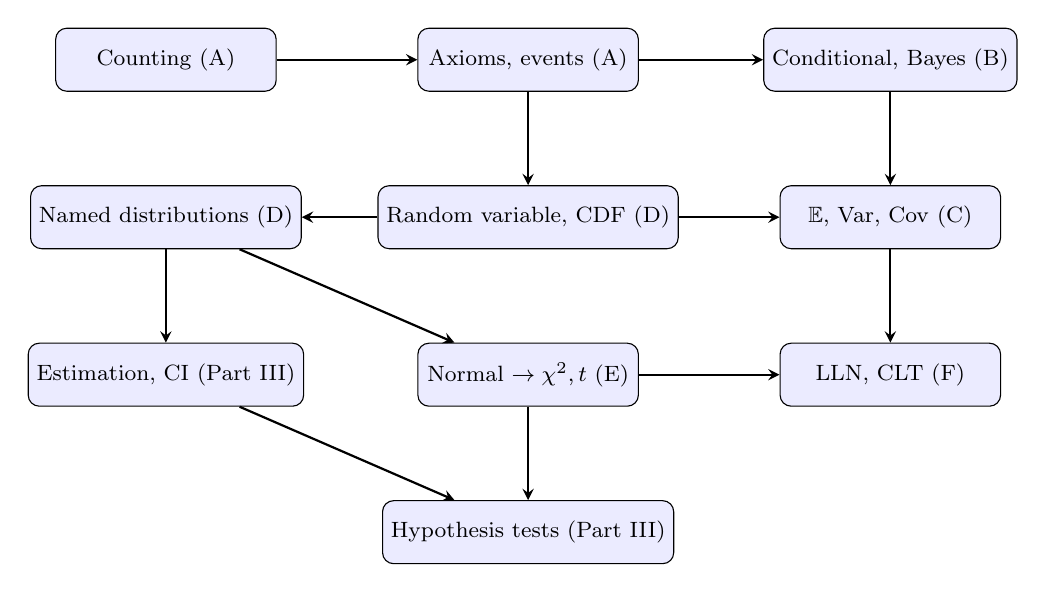
\begin{tikzpicture}[
 b/.style={draw,rounded corners,fill=blue!8,minimum height=8mm,minimum width=28mm,align=center,font=\footnotesize,inner sep=3pt},
 a/.style={->,thick,>=stealth}]
\node[b] (cnt) at (0,0) {Counting (A)};
\node[b] (ax) at (4.6,0) {Axioms, events (A)};
\node[b] (cond) at (9.2,0) {Conditional, Bayes (B)};
\node[b] (dist) at (0,-2) {Named distributions (D)};
\node[b] (rv) at (4.6,-2) {Random variable, CDF (D)};
\node[b] (ev) at (9.2,-2) {$\E$, $\Var$, $\Cov$ (C)};
\node[b] (est) at (0,-4) {Estimation, CI (Part III)};
\node[b] (nor) at (4.6,-4) {Normal $\to\chi^2,t$ (E)};
\node[b] (clt) at (9.2,-4) {LLN, CLT (F)};
\node[b] (tst) at (4.6,-6) {Hypothesis tests (Part III)};
\draw[a](cnt)--(ax);\draw[a](ax)--(cond);\draw[a](ax)--(rv);\draw[a](cond)--(ev);
\draw[a](rv)--(ev);\draw[a](rv)--(dist);\draw[a](dist)--(nor);\draw[a](ev)--(clt);
\draw[a](nor)--(clt);\draw[a](dist)--(est);\draw[a](est)--(tst);\draw[a](nor)--(tst);
\end{tikzpicture}
\end{center}
Read the arrows as ``is needed for''. Every question below is tagged with the box it belongs to.

% =====================================================================
\section{Group A: Counting and Basic Probability (6 questions)}

\begin{story}[The complement trick]
Ramu: ``What is the chance that at least one of 100 dice shows a 1? Adding up cases is impossible.'' Somu: ``Do the opposite: compute the chance that \emph{none} shows a 1, then subtract from 1.'' The same trick solves half of all counting-probability questions.
\end{story}

\begin{example}[2025 Q45 (2 marks, MCQ): at least one 1 among 100 dice]
Each die avoids a 1 with probability $5/6$, independently. $\Pr(\text{none})=(5/6)^{100}$, so
\[\Pr(A)=1-(5/6)^{100}\approx0.99999999\quad\Rightarrow\ \textbf{(C)}.\]
\textbf{Connect:} complement rule (Axioms chapter) $+$ independence (Conditional chapter). The same trick appears in the birthday problem and in ``at least one defective item'' questions.
\end{example}

\begin{example}[2024 Q12 (1 mark, MCQ): two events that cannot happen together]
Three fair coins. $T$: at least two heads. $S$: at least two tails. Both would need $\ge4$ coins, so $T\cap S=\emptyset$ and $\Pr(T\cap S)=\mathbf0$ \quad (A).\\
\textbf{Connect:} $T$ and $S$ are \emph{mutually exclusive}, which is not the same as independent (here $\Pr(T)\Pr(S)=\tfrac12\cdot\tfrac12\neq0$, so they are in fact dependent).
\end{example}

\begin{example}[2026 Q19 (1 mark, MCQ): a random subset has an even product]
$M$ is a uniformly random \emph{non-empty} subset of $\{1,\dots,2026\}$. The product is odd only if every element is odd. There are $1013$ odd numbers, so $2^{1013}-1$ non-empty all-odd subsets, out of $2^{2026}-1$ non-empty subsets.
\[\Pr(\text{even})=1-\frac{2^{1013}-1}{2^{2026}-1}=\frac{2^{2026}-2^{1013}}{2^{2026}-1}=\frac{2^{1013}(2^{1013}-1)}{2^{2026}-1}\quad\Rightarrow\ \textbf{(C)}.\]
\textbf{Trap:} the word ``non-empty'' changes the denominator to $2^{2026}-1$ (options A and B forget it). \textbf{Check:} for $N=4$ the formula gives $\frac{4\cdot3}{15}=\frac45$, and brute force over all $15$ non-empty subsets gives $12/15$.
\end{example}

\begin{example}[2026 Q20 (1 mark, MCQ): all four numbers positive]
A program returns a non-negative integer solution of $n_1+n_2+n_3+n_4=20$, each solution equally likely. By \textbf{stars and bars}, the number of non-negative solutions is $\binom{20+3}{3}=\binom{23}{3}=1771$. Positive solutions: put $m_i=n_i-1\ge0$, giving $m_1+\dots+m_4=16$, so $\binom{19}{3}=969$. Hence
\[\Pr=\frac{\binom{19}{3}}{\binom{23}{3}}=\frac{969}{1771}\approx0.547\quad\Rightarrow\ \textbf{(A)}.\]
\textbf{Connect:} stars and bars is in the Counting chapter; ``positive'' means subtract $1$ from each variable first.
\end{example}

\begin{example}[2026 Q33 (1 mark, NAT): functions that undo themselves]
Count bijections $f$ on $\{1,2,3,4\}$ with $f(f(x))=x$ for every $x$ (these are \textbf{involutions}: identity and products of disjoint swaps). Count by number of swaps:
\begin{itemize}[noitemsep]
\item $0$ swaps: identity, $1$ way. \quad $1$ swap: $\binom42=6$ ways.
\item $2$ swaps: split $4$ items into two pairs, $\frac{\binom42\binom22}{2}=3$ ways.
\end{itemize}
Total $1+6+3=\mathbf{10}$. (Recurrence check: $a_n=a_{n-1}+(n-1)a_{n-2}$ with $a_1=1,a_2=2$ gives $a_3=4$ and $a_4=4+3\cdot2=10$.) Verified by listing all $24$ permutations.\\
\textbf{Connect:} counting with permutations (Counting chapter); no probability needed, it is a pure combinatorics question.
\end{example}

\begin{example}[2026 Q64 (2 marks, NAT): a $5\times5$ random 0/1 matrix]
Entries are independent Bernoulli$(0.5)$. Want $\Pr(\text{row 2 sums to }3\ \text{and column 3 sums to }3)$. Row $2$ and column $3$ share the entry in position $(2,3)$, so they are \emph{not} independent. \textbf{Condition on the shared cell} $c$:
\begin{itemize}[noitemsep]
\item $c=1$ (prob.\ $\tfrac12$): the other $4$ cells of the row need two $1$s and the other $4$ of the column need two $1$s: $\bigl(\binom42/16\bigr)^2=(6/16)^2$.
\item $c=0$ (prob.\ $\tfrac12$): each needs three $1$s among $4$ cells: $\bigl(\binom43/16\bigr)^2=(4/16)^2$.
\end{itemize}
\[\Pr=\tfrac12\Bigl(\tfrac{36}{256}+\tfrac{16}{256}\Bigr)=\tfrac{26}{256}=\mathbf{0.1016}\approx0.10\]
(official range $0.08$ to $0.12$). A simulation of $10^6$ matrices gave $0.1015$.\\
\textbf{Lesson:} when two events overlap in one random variable, \textbf{condition on the overlap}, then everything else is independent.
\end{example}

% =====================================================================
\section{Group B: Conditional Probability and Bayes (3 questions)}

\begin{story}[Always draw the tree]
Ramu: ``A test is 80\% accurate for sick people. If I test positive, am I 80\% likely to be sick?'' Somu: ``No: that is $\Pr(+\mid\text{sick})$, but you want $\Pr(\text{sick}\mid+)$. They are different, and the difference depends on how rare the sickness is.'' All three questions here are this idea.
\end{story}

\begin{formula}[Bayes in two forms]
\[\Pr(A_i\mid B)=\frac{\Pr(B\mid A_i)\Pr(A_i)}{\sum_j\Pr(B\mid A_j)\Pr(A_j)}\qquad\text{(denominator = total probability)}\]
\textbf{Odds form:} posterior odds $=$ prior odds $\times$ likelihood ratio.
\end{formula}

\begin{example}[2026 Q57 (2 marks, NAT): medical test]
$\Pr(D)=0.3$, $\Pr(+\mid D)=0.8$, $\Pr(+\mid\neg D)=0.1$.
\[\Pr(D\mid+)=\frac{0.8\cdot0.3}{0.8\cdot0.3+0.1\cdot0.7}=\frac{0.24}{0.31}=\mathbf{0.774}\quad(\text{key: }0.76\text{ to }0.78).\]
Odds check: prior odds $\frac{0.3}{0.7}=\frac37$, likelihood ratio $\frac{0.8}{0.1}=8$, posterior odds $\frac{24}{7}$, probability $\frac{24}{31}=0.774$. Note the false-positive column ($0.1$) uses the \emph{healthy} $70\%$.
\end{example}

\begin{example}[2025 Q31 (1 mark, NAT): three boxes]
Priors $\tfrac12,\tfrac16,\tfrac13$; white-ball chances $\tfrac13,\tfrac23,\tfrac12$.
\[\Pr(W)=\tfrac12\cdot\tfrac13+\tfrac16\cdot\tfrac23+\tfrac13\cdot\tfrac12=\tfrac16+\tfrac19+\tfrac16=\tfrac49,\qquad\Pr(\text{Box 2}\mid W)=\frac{1/9}{4/9}=\mathbf{0.25}.\]
Note the priors are \emph{not} equal, a favourite trap: do not assume each box is picked with probability $1/3$.
\end{example}

\begin{example}[2024 Q58 (2 marks, NAT): events $T$ and $S$]
Given $\Pr(\bar T)=0.6$ (so $\Pr(T)=0.4$), $\Pr(S\mid T)=0.3$, $\Pr(S\mid\bar T)=0.6$.
\[\Pr(S)=0.4\cdot0.3+0.6\cdot0.6=0.12+0.36=0.48,\qquad \Pr(T\mid S)=\frac{0.12}{0.48}=\mathbf{0.25}.\]
\textbf{Trap:} the problem gives $\Pr(\bar T)$, not $\Pr(T)$.
\end{example}

\begin{intuition}
\textbf{Connected question from the ML section: 2025 Q35 (naive Bayes).}
Priors $\tfrac13,\tfrac23$; likelihoods $\tfrac34,\tfrac14$ for the feature vector $x$. Posterior numerators: $\tfrac14$ and $\tfrac16$, total $\tfrac5{12}$, so the posteriors are $0.6$ and $0.4$. The classifier picks class $1$, so the \textbf{misclassification probability is $0.4$}. A naive-Bayes classifier is nothing but Bayes' theorem followed by ``pick the largest posterior''. This is the bridge between this chapter and the Machine Learning notes.
\end{intuition}

% =====================================================================
\section{Group C: Expectation, Variance, Covariance (10 questions)}

\begin{story}[Variance is the spread, and it does not care about shifts]
Ramu: ``If every student gets $5$ bonus marks, does the class spread change?'' Somu: ``No. Shifting does not change the spread, but \emph{multiplying} by $a$ multiplies the variance by $a^2$.'' Many questions below hide this rule: $\Var(aX+b)=a^2\Var(X)$.
\end{story}

\begin{formula}[Rules used in Group C]
\begin{itemize}[noitemsep]
\item $\E[aX+b]=a\E[X]+b$ always (linearity, even for dependent variables). $\Var(aX+b)=a^2\Var(X)$.
\item $\Var(X)=\E[X^2]-(\E X)^2$; \quad $\Cov(X,Y)=\E[XY]-\E[X]\E[Y]$; independence $\Rightarrow\Cov=0$ (not conversely).
\item \textbf{Law of iterated expectation:} $\E[\E[X\mid Y]]=\E[X]$.
\item Independent $X,Y$: $\Var(XY)=\E[X^2]\E[Y^2]-(\E X)^2(\E Y)^2$.
\item Bernoulli$(p)$: mean $p$, variance $p(1-p)$; Binomial$(n,p)$: mean $np$, variance $np(1-p)$.
\end{itemize}
\end{formula}

\begin{example}[2025 Q11 (1 mark, MCQ): law of iterated expectation]
$\E[\E[X\mid Y]]=\E[X]$ \quad (C). Reason: first average inside each value of $Y$, then average those averages with weights $\Pr(Y=y)$, which gives the overall average. A proof is in Part III.
\end{example}

\begin{example}[2025 Q20 (1 mark, MCQ): $X=aZ+b$]
Given $\E[X]=1$, $\E[(X-\E X)Z]=-2$, $\E[(X-\E X)^2]=4$, and $Z\sim N(0,1)$.
\begin{itemize}[noitemsep]
\item $\E[X]=a\cdot0+b=b$, so $b=1$.
\item $\Var(X)=a^2=4\Rightarrow a=\pm2$.
\item $\E[(X-1)Z]=\E[aZ^2]=a\cdot1=-2\Rightarrow a=-2$. This second condition \emph{fixes the sign}.
\end{itemize}
Answer: $a=-2,\ b=1$ \quad (A).
\end{example}

\begin{example}[2025 Q54 (2 marks, MSQ): the sample proportion]
$\hat p=\frac1n\sum X_i$ with $X_i\sim\text{Bernoulli}(p)$ independent. $\E[\hat p]=\frac1n\cdot np=p$ (so \textbf{A} true, B false), and $\Var(\hat p)=\frac1{n^2}\cdot np(1-p)=\frac{p(1-p)}{n}$, which \textbf{decreases} with $n$ (C true, D false). Answer: A, C. This is the law of large numbers in one line: the estimator is unbiased and its spread shrinks like $1/n$.
\end{example}

\begin{example}[2025 Q61 (2 marks, NAT): black balls with replacement]
$5$ white and $10$ black, so $\Pr(\text{black})=\frac{10}{15}=\frac23$. $S_{100}\sim\text{Bin}(100,\tfrac23)$, $\E[S_{100}]=\frac{200}{3}=\mathbf{66.7}$ (key: $66.6$ to $66.7$). By linearity you do not even need the binomial: $100$ draws, each contributing $\frac23$.
\end{example}

\begin{example}[2024 Q34 (1 mark, NAT): updating an average]
$50$ points with average $40$ have total $2000$. Add $142$: total $2142$ over $51$ points, new mean $=\frac{2142}{51}=\mathbf{42}$. (Shortcut: the new point is $102$ above the old mean, spread over $51$ points adds $2$.)
\end{example}

\begin{example}[2024 Q36 (2 marks, MCQ): throws until two evens in a row]
A fair die is even with probability $\frac12$. Let $a$ be the expected number of throws from the start (last throw not even) and $b$ the expected number after one even throw.
\[a=1+\tfrac12 b+\tfrac12 a,\qquad b=1+\tfrac12\cdot0+\tfrac12 a.\]
From the first: $a=2+b$. Substituting $b=1+\tfrac a2$: $a=3+\tfrac a2\Rightarrow a=\mathbf6$ \quad (C). For a general coin, the expected waiting time for two consecutive successes is $\frac{1+p}{p^2}=\frac{1.5}{0.25}=6$.\\
\textbf{Technique:} set up states and write one equation per state (\emph{first-step analysis}).
\end{example}

\begin{example}[2024 Q65 (2 marks, NAT): covariance of two coin variables]
Two fair coins: $X=1$ if both heads, $Y=1$ if at least one head. Outcomes: HH $(1,1)$, HT $(0,1)$, TH $(0,1)$, TT $(0,0)$, each $\frac14$.
\[\E X=\tfrac14,\quad\E Y=\tfrac34,\quad\E[XY]=\tfrac14\ (\text{only HH}),\quad\Cov=\tfrac14-\tfrac14\cdot\tfrac34=\tfrac1{16}=\mathbf{0.0625}.\]
Key range $0.062$ to $0.063$. $X$ and $Y$ are positively correlated: $X=1$ forces $Y=1$.
\end{example}

\begin{example}[2026 Q44 (2 marks, MCQ): variance of $(2X-1)Y$]
$X\sim\text{Bernoulli}(0.3)$, $Y\sim N(0,100)$, independent. The trick: $2X-1$ is $+1$ when $X=1$ and $-1$ when $X=0$, so $(2X-1)^2=1$ \emph{always}. Then $\E[(2X-1)Y]=\E[2X-1]\E[Y]=0$ and
\[\Var=\E[(2X-1)^2Y^2]=\E[Y^2]=100\quad\Rightarrow\ \textbf{(A)}.\]
(Simulation gave $99.96$.) The product-variance formula agrees: $\E[(2X-1)^2]\E[Y^2]-0=1\cdot100$.
\end{example}

\begin{example}[2026 Q62 (2 marks, NAT): pairwise differences and the variance]
For $n=100$: $\frac1{2000}\sum_{i,j}(x_i-x_j)^2=99$. Identity: $\sum_{i,j}(x_i-x_j)^2=2n\sum_i(x_i-\bar x)^2$. So
\[\frac{200}{2000}\sum_i(x_i-\bar x)^2=99\ \Rightarrow\ \sum_i(x_i-\bar x)^2=990,\qquad s^2=\frac{990}{99}=\mathbf{10}.\]
(Verified numerically on random data.) The identity is proved in Part III.
\end{example}

\begin{example}[2026 Q63 (2 marks, NAT): correlation of $X$ and $Y\mid X$]
$X\sim U(-1,1)$; given $X=x$, $Y\sim U(x^2-0.1,\,x^2+0.1)$, so $\E[Y\mid X]=X^2$. Then
\[\Cov(X,Y)=\E[XY]-\E X\,\E Y=\E\bigl[X\,\E[Y\mid X]\bigr]-0=\E[X^3]=0.\]
Correlation $=\mathbf0$ (answer key: $0$) even though $Y$ depends strongly on $X$: \textbf{uncorrelated does not mean independent}. The proof uses the law of iterated expectation of the previous list.
\end{example}

\begin{trap}
(1) $\Var(aX+b)$ has no $b$ and uses $a^2$. (2) Zero covariance does not give independence (2026 Q63). (3) Do not divide $\hat p$'s expectation by $n$ (2025 Q54-B). (4) In MSQ, mark \emph{all} true statements; a missed one earns zero.
\end{trap}

% =====================================================================
\section{Group D: Distributions, CDF, Joint Density (10 questions)}

\begin{story}[A CDF is the whole story in one curve]
Ramu: ``Why do GATE questions give a CDF with a constant $t$ and ask for the median?'' Somu: ``The median is the value $m$ with $F(m)=\tfrac12$. Once you can read probabilities from a CDF, intervals, medians and transformed events are all just subtractions.''
\end{story}

\begin{formula}[CDF facts]
$F(x)=\Pr(X\le x)$ is non-decreasing, right-continuous, $F(-\infty)=0$, $F(\infty)=1$. $\Pr(a<X\le b)=F(b)-F(a)$. Discrete $X$: $F$ is a step function with jumps equal to the pmf values. Median $m$: $F(m)=\tfrac12$. Exponential with rate $\lambda$: $F(x)=1-e^{-\lambda x}$, mean $\tfrac1\lambda$, variance $\tfrac1{\lambda^2}$, \textbf{memoryless}: $\Pr(X>s+t\mid X>s)=\Pr(X>t)$.
\end{formula}

\begin{example}[2025 Q19 (1 mark, MCQ): median from a CDF with a constant]
$F(x)=\dfrac{x-t}{4-t}$ on $[t,4]$. Median $3$ means $F(3)=\tfrac12$: $\dfrac{3-t}{4-t}=\dfrac12\Rightarrow 6-2t=4-t\Rightarrow t=\mathbf2$ \quad (A).
\end{example}

\begin{example}[2025 Q39 (2 marks, MCQ): probability of $X^2\le0.25$]
$F(x)=\frac14(x+1)^2$ on $[-1,1]$. $X^2\le0.25\iff-0.5\le X\le0.5$:
\[F(0.5)-F(-0.5)=\tfrac14(1.5)^2-\tfrac14(0.5)^2=\tfrac{2.25-0.25}{4}=\mathbf{0.5}\quad(\text{C}).\]
\textbf{Technique:} translate the event on $g(X)$ into an interval for $X$, then subtract CDF values.
\end{example}

\begin{example}[2025 Q21 (1 mark, MCQ) and 2026 Q34 (1 mark, NAT): exponential tails]
\textbf{2025 Q21:} $\Pr(X\ge2)=e^{-2\lambda}=0.25\Rightarrow2\lambda=\ln4\Rightarrow\lambda=\ln2$ \quad (A).\\
\textbf{2026 Q34:} $X$ is exponential with mean $\lambda$ and $\Pr(X>5)=0.35$. By \textbf{memorylessness},
$\Pr(X>10\mid X>5)=\Pr(X>5)=\mathbf{0.35}$ (key: $0.34$ to $0.36$). No parameter needed.\\
\textbf{Watch out:} in 2025 Q21 the mean is $1/\lambda$ (rate form), in 2026 Q34 the mean is the parameter itself. Always read how the question parametrises the exponential.
\end{example}

\begin{example}[2025 Q41 (2 marks, MCQ): the integer part of an exponential is geometric]
$X\sim\text{Exp}(\lambda=\ln10)$, $Y=\lfloor X\rfloor$. Then $\Pr(Y\ge\ell)=\Pr(X\ge\ell)=e^{-\lambda\ell}=10^{-\ell}$, so
\[\Pr(Y=\ell)=10^{-\ell}-10^{-(\ell+1)}=(0.1)^\ell(0.9)\ \Rightarrow\ q=\mathbf{0.1}\quad(\text{A}).\]
In general $q=e^{-\lambda}$, and $Y\sim\text{Geometric}$ (number of failures before the first success). \textbf{Connect:} this links the continuous exponential to the discrete geometric; both are memoryless.
\end{example}

\begin{example}[2024 Q57 (2 marks, NAT): when does $5\,\E X=\Var X$?]
Exponential with rate $\lambda$: $\E X=\tfrac1\lambda$, $\Var X=\tfrac1{\lambda^2}$. $\tfrac5\lambda=\tfrac1{\lambda^2}\Rightarrow\lambda=\tfrac15=\mathbf{0.2}$.
\end{example}

\begin{example}[2024 Q56 (2 marks, NAT): $\Pr(X\ge Y)$ for two independent uniforms]
$X\sim U[1,3]$, $Y\sim U[2,4]$; joint density $\frac12\cdot\frac12=\frac14$ on the square $[1,3]\times[2,4]$ (area $4$). $X\ge Y$ requires $X\ge2$ and $Y\le X$: the region inside the square is the triangle with corners $(2,2),(3,2),(3,3)$, area $\frac12$. $\Pr=\frac14\cdot\frac12=\mathbf{0.125}$. Simulation: $0.1248$.
\end{example}

\begin{example}[{2024 Q59 (2 marks, NAT; MTA): $\E[Y\mid X=1.5]$}]
Joint density $2xy$ on $0<y<x<2$. Conditional density of $Y$ given $X=x$: $\dfrac{2xy}{\int_0^x2xy\,dy}=\dfrac{2y}{x^2}$ on $0<y<x$. So
\[\E[Y\mid X=x]=\int_0^xy\cdot\frac{2y}{x^2}dy=\frac{2x}{3}\ \Rightarrow\ \E[Y\mid X=1.5]=\mathbf1.\]
The method needs only the \emph{shape} of the density (normalisation cancels), but the given density integrates to $4$ over the region, which is why the key says MTA.
\end{example}

\begin{example}[2024 Q11 (1 mark, MCQ) and 2026 Q54 (2 marks, MSQ)]
\textbf{2024 Q11:} Poisson: mean $=$ variance $=\lambda$ (true); standard normal: mean $0$, variance $1$ (true). Both true \quad (A).\\
\textbf{2026 Q54 (discrete CDF):} (A) $F>0$ always: \emph{false} ($F=0$ below the smallest value). (B) non-decreasing: \textbf{true}. (C) has jump discontinuities: \textbf{true} (a discrete variable's CDF jumps at each support point). (D) left-continuous: \emph{false} (CDFs are \emph{right}-continuous). Answer: B, C.
\end{example}

% =====================================================================
\section{Group E: The Normal Family ($\chi^2$, $t$) (3 questions)}

\begin{story}[Squares of bell curves]
Ramu: ``Why does everybody keep squaring normals?'' Somu: ``Because spread is measured by squares. Add up $n$ squared standard normals and you get a $\chi^2_n$. Divide a normal by the square root of a $\chi^2$ and you get a $t$. These two facts power every test in the syllabus.''
\end{story}

\begin{formula}[Facts to memorise]
\begin{itemize}[noitemsep]
\item $Z_i$ i.i.d.\ $N(0,1)$: $\sum_{i=1}^nZ_i^2\sim\chi^2_n$, with mean $n$ and variance $2n$.
\item $\chi^2_2$ is exactly Exponential with mean $2$. \quad $\chi^2_1=Z^2$.
\item $X_i$ i.i.d.\ $N(\mu,\sigma^2)$: $\bar X$ and $\sum(X_i-\bar X)^2$ are \textbf{independent}, and $\dfrac{\sum(X_i-\bar X)^2}{\sigma^2}\sim\chi^2_{n-1}$ (one degree of freedom is lost estimating the mean).
\item $T=\dfrac{Z}{\sqrt{\chi^2_k/k}}\sim t_k$. $t_1$ is the \textbf{Cauchy} distribution. $t_k\to N(0,1)$ as $k\to\infty$. Pdf is symmetric about $0$ with \textbf{heavier tails} than the normal.
\end{itemize}
\end{formula}

\begin{example}[2025 Q36 (2 marks, MCQ): $\Var(Z^2)$ for standard normal $Z$]
$\Var(Z^2)=\E[Z^4]-(\E Z^2)^2=3-1=\mathbf2$ \quad (B). Equivalently $Z^2\sim\chi^2_1$ with variance $2\cdot1=2$. Simulation: $2.001$.
\end{example}

\begin{example}[2026 Q53 (2 marks, MSQ): four statements on normal samples]
$X_1,\dots,X_n$ i.i.d.\ $N(0,1)$.
\begin{itemize}[noitemsep]
\item (A) $\sum X_i^2\sim\chi^2_n$: \textbf{true} (definition).
\item (B) $\sum(X_i-\bar X)^2\sim\chi^2_{n-1}$: \textbf{true} (one df lost).
\item (C) $X_1^2+X_n^2\sim$ Exponential with mean $2$: \textbf{true} since $\chi^2_2$ is exponential with mean $2$.
\item (D) $(\sqrt n\bar X)^2\sim\chi^2_2$: \emph{false}. $\sqrt n\bar X\sim N(0,1)$, so its square is $\chi^2_1$.
\end{itemize}
Answer: A, B, C. Simulation with $n=5$: (B) had mean $4.00$, variance $8.0$ ($\chi^2_4$: $4,8$); (C) mean $2.00$, variance $4.0$ (Exp(mean 2): $2,4$); (D) mean $1.0$, variance $2.0$ ($\chi^2_1$).
\end{example}

\begin{example}[2026 Q28 (1 mark, MSQ): normal versus $t_1$]
$g,G$ are the standard normal pdf, cdf; $h,H$ those of $t_1$ (Cauchy, $h(x)=\frac1{\pi(1+x^2)}$); $c>0$ with $g(c)=h(c)$ ($c\approx1.851$).
\begin{itemize}[noitemsep]
\item (A) $G(0)=H(0)$: \textbf{true}, both symmetric about $0$, so both equal $\tfrac12$.
\item (D) $g(0)=h(0)$: \emph{false}; $g(0)=0.399$ but $h(0)=1/\pi=0.318$ (the normal is more peaked).
\item Beyond $c$ the $t_1$ density is above the normal's (heavier tails). So the upper tail $1-H(c)>1-G(c)$, i.e.\ $H(c)<G(c)$: (B) $G(c)<H(c)$ is \emph{false} ($G(c)=0.968$, $H(c)=0.842$).
\item By symmetry the lower tail is bigger for $t_1$: $G(-c)=0.032<H(-c)=0.158$: (C) \textbf{true}.
\end{itemize}
Answer: A, C. \textbf{Idea:} ``heavy tails'' means more probability far from the centre, hence the $t$ critical values ($12.7$ at $df=1$, $2.57$ at $df=5$) exceed $1.96$.
\end{example}

% =====================================================================
\section{Group F: CLT and Limits (2 questions)}

\begin{example}[2025 Q40 (2 marks, MCQ): CLT for $300$ Bernoulli variables]
$Y=\sum_{i=1}^{300}X_i$, $X_i\sim\text{Bernoulli}(0.25)$. $\E Y=300\cdot0.25=75$, $\Var Y=300\cdot0.25\cdot0.75=56.25$, $\sigma=7.5$. For $\Pr(60\le Y\le90)$:
\[\frac{60-75}{7.5}=-2,\qquad\frac{90-75}{7.5}=+2\ \Rightarrow\ \Pr\approx\Phi(2)-\Phi(-2)\quad\textbf{(A)}\ (\approx0.954).\]
The exact binomial probability is $0.962$, so the approximation is good. \textbf{Always} compute mean and standard deviation first; the options are decoys with wrong $z$-values.
\end{example}

\begin{example}[2026 Q45 (2 marks, MCQ): a Poisson sum that tends to $\tfrac12$]
$\sum_{k=0}^ne^{-n}\frac{n^k}{k!}=\Pr(N_n\le n)$ where $N_n\sim\text{Poisson}(n)$ (mean $n$, variance $n$). By the CLT $N_n\approx N(n,n)$, and $\Pr(N_n\le n)\to\Pr(Z\le0)=\tfrac12$. Exact values: $n=10$: $0.583$; $n=100$: $0.527$; $n=1000$: $0.508$; $n=10000$: $0.503$. So $L=\mathbf{0.5}$ \quad (A).\\
\textbf{Connect:} a Poisson$(n)$ is a sum of $n$ independent Poisson$(1)$ variables, so the CLT applies. The slow convergence comes from the discreteness (a continuity correction explains the leftover $\approx\frac{1}{\sqrt{2\pi n}}\cdot\frac12$).
\end{example}

% =====================================================================
\section{Eight Tricks that Solved Most of These 34 Questions}
\begin{formula}[Connecting the dots]
\begin{enumerate}[noitemsep]
\item \textbf{Complement:} ``at least one'' $=1-\Pr(\text{none})$ (2025 Q45, 2026 Q19).
\item \textbf{Condition on the overlap} of dependent events (2026 Q64).
\item \textbf{Bayes tree}: priors $\times$ likelihoods, divide by the total (2024 Q58, 2025 Q31, 2026 Q57, 2025 Q35).
\item \textbf{First-step analysis}: one equation per state (2024 Q36).
\item \textbf{Linearity of expectation} and $\Var(aX+b)=a^2\Var X$ (2025 Q54, Q61, 2026 Q44).
\item \textbf{Law of iterated expectation}: $\E[g(X)\,\E[Y|X]]$ (2025 Q11, 2026 Q63, 2024 Q59).
\item \textbf{Memorylessness and the CDF}: $F(x)=1-e^{-\lambda x}$ turns every exponential question into algebra (2025 Q21, Q41; 2026 Q34; 2024 Q57).
\item \textbf{Normal family and CLT}: $\chi^2_n$ has mean $n$, variance $2n$; $t$ has heavy tails; standardise before using the CLT (2025 Q36, Q40; 2026 Q28, Q45, Q53).
\end{enumerate}
\end{formula}

\begin{center}
\small
\begin{tabularx}{\textwidth}{>{\raggedright\arraybackslash}p{2.3cm}>{\raggedright\arraybackslash}X>{\raggedright\arraybackslash}p{3.2cm}}
\toprule
\textbf{Question} & \textbf{Idea in one line} & \textbf{Notes chapter}\\\midrule
24-Q11 (A) & Poisson mean=variance; $N(0,1)$ & Common distributions\\
24-Q12 (A, $0$) & events can't both occur & Axioms\\
24-Q34 ($42$) & total / count & Random variables\\
24-Q36 (C, $6$) & first-step equations & Expectation\\
24-Q56 ($0.125$) & area of region $\times$ density & Joint distributions\\
24-Q57 ($0.2$) & $5/\lambda=1/\lambda^2$ & Continuous distributions\\
24-Q58 ($0.25$) & Bayes & Bayes\\
24-Q59 (MTA, $1$) & $\E[Y|X]$ from joint density & Joint distributions\\
24-Q65 ($0.0625$) & $\E[XY]-\E X\E Y$ & Covariance\\
25-Q11 (C) & $\E[\E[X|Y]]=\E X$ & Expectation\\
25-Q19 (A, $t=2$) & median: $F(m)=\frac12$ & CDF\\
25-Q20 (A) & $\Var(aZ+b)$, covariance sign & Normal\\
25-Q21 (A) & $e^{-2\lambda}=0.25$ & Exponential\\
25-Q31 ($0.25$) & Bayes & Bayes\\
25-Q36 (B, $2$) & $\Var(\chi^2_1)=2$ & Normal family\\
25-Q39 (C, $0.5$) & $F(0.5)-F(-0.5)$ & CDF\\
25-Q40 (A) & CLT, $z=\pm2$ & CLT\\
25-Q41 (A, $0.1$) & floor of exponential & Exponential, Geometric\\
25-Q45 (C) & complement & Axioms\\
25-Q54 (A,C) & $\Var\hat p=p(1-p)/n$ & Estimation\\
25-Q61 ($66.7$) & $np$ & Binomial\\
26-Q19 (C) & complement, non-empty & Counting\\
26-Q20 (A) & stars and bars & Counting\\
26-Q28 (A,C) & heavy tails & Normal family\\
26-Q33 ($10$) & involutions & Counting\\
26-Q34 ($0.35$) & memoryless & Exponential\\
26-Q44 (A, $100$) & $(2X-1)^2=1$ & Variance\\
26-Q45 (A, $0.5$) & Poisson$(n)$ and CLT & CLT\\
26-Q53 (A,B,C) & $\chi^2$ facts & Normal family\\
26-Q54 (B,C) & discrete CDF & CDF\\
26-Q57 ($0.774$) & Bayes & Bayes\\
26-Q62 ($10$) & pairwise identity & Sample variance\\
26-Q63 ($0$) & $\E[X^3]=0$ & Covariance\\
26-Q64 ($0.10$) & condition on shared cell & Independence\\
\bottomrule
\end{tabularx}
\end{center}
\textbf{Sample-paper bonus (GATE 2024 DA sample paper, Q7):} a fair coin is flipped twice and at least one tail is known. Sample space reduces to $\{HT,TH,TT\}$, so $\Pr(\text{two tails})=\tfrac13$, an example of conditioning as restriction.

% =====================================================================
\newpage
\part{Deeper Explanations: Proofs and Intuition}

\section{Why the Key Formulas are True}

\begin{story}[Ramu insists on ``why'']
Ramu: ``I can use $\E[\E[X|Y]]=\E[X]$ but I do not believe it.'' Somu: ``Then let us prove each one slowly.''
\end{story}

\subsection{Law of iterated expectation and total variance}
\begin{formula}[Statement and proof]
For discrete $Y$: $\E[X\mid Y=y]=\sum_xx\Pr(X=x\mid Y=y)$ is a function of $y$. Then
\begin{align*}\E[\E[X\mid Y]]&=\sum_y\Pr(Y=y)\sum_xx\frac{\Pr(X=x,Y=y)}{\Pr(Y=y)}\\&=\sum_x x\sum_y\Pr(X=x,Y=y)=\sum_xx\Pr(X=x)=\E[X].\end{align*}
\textbf{Total variance:} $\Var(X)=\E[\Var(X\mid Y)]+\Var(\E[X\mid Y])$ (average within-group spread plus spread of the group means). \textbf{Everyday picture:} the average marks of the whole college is the weighted average of the class averages.
\end{formula}
\begin{example}[Using it: 2026 Q63 in two lines]
$\Cov(X,Y)=\E[XY]-\E X\E Y$ and $\E[XY]=\E[\E[XY\mid X]]=\E[X\,\E[Y\mid X]]=\E[X\cdot X^2]=\E[X^3]=0$ because $X\sim U(-1,1)$ is symmetric. Also $\E X=0$. So the covariance is $0$.
\end{example}

\subsection{Variance of products and the sample-variance identity}
\begin{formula}[Two identities]
\textbf{(i) Independent $X,Y$:} $\Var(XY)=\E[X^2]\E[Y^2]-(\E X)^2(\E Y)^2$, because $\E[(XY)^2]=\E[X^2]\E[Y^2]$ and $\E[XY]=\E X\E Y$.\\
\textbf{(ii) Pairwise differences:}
\begin{align*}\sum_{i,j}(x_i-x_j)^2&=\sum_{i,j}\bigl[(x_i-\bar x)-(x_j-\bar x)\bigr]^2\\&=n\sum_i(x_i-\bar x)^2+n\sum_j(x_j-\bar x)^2-2\Bigl(\sum_i(x_i-\bar x)\Bigr)^2\\&=2n\sum_i(x_i-\bar x)^2.\end{align*}
(the cross term vanishes since $\sum(x_i-\bar x)=0$). Hence the sample variance is \(s^2=\dfrac{1}{n-1}\sum_i(x_i-\bar x)^2=\dfrac{1}{2n(n-1)}\sum_{i,j}(x_i-x_j)^2\). For $n=100$ this is $\frac{1}{19800}\sum_{i,j}(x_i-x_j)^2$, which is how 2026 Q62 reduces to $s^2=10$.
\end{formula}

\subsection{Why the exponential is memoryless, and where it comes from}
\begin{formula}[Memorylessness proof]
$\Pr(X>s+t\mid X>s)=\dfrac{e^{-\lambda(s+t)}}{e^{-\lambda s}}=e^{-\lambda t}=\Pr(X>t)$. It is the \emph{only} continuous distribution with this property (the geometric is the only discrete one).\\
\textbf{Origin:} if events happen at a constant average rate $\lambda$ (a Poisson process), the number of events in time $t$ is Poisson$(\lambda t)$, and the waiting time to the first event has $\Pr(X>t)=\Pr(\text{no events})=e^{-\lambda t}$, which is the exponential tail. This unifies Poisson, exponential and (by counting whole periods) geometric.
\end{formula}
\begin{formula}[Poisson as the limit of the binomial]
$n$ large, $p$ small, $np=\lambda$: $\binom nk p^k(1-p)^{n-k}\to e^{-\lambda}\lambda^k/k!$. Check: $\text{Bin}(1000,0.003)$ gives $\Pr(X=2)=0.2242$ and Poisson$(3)$ gives $0.2240$.
\end{formula}

\subsection{Normal, $\chi^2$ and $t$: where they come from}
\begin{formula}[A chain of three ideas]
\begin{enumerate}[noitemsep]
\item $Z\sim N(0,1)\Rightarrow Z^2$ has $\E=1$, $\E Z^4=3$, so $\Var(Z^2)=2$.
\item Adding independent $\chi^2$ variables adds degrees of freedom: $\chi^2_a+\chi^2_b=\chi^2_{a+b}$. So $\sum_{i=1}^nZ_i^2\sim\chi^2_n$.
\item Sample variance: $\frac{(n-1)S^2}{\sigma^2}\sim\chi^2_{n-1}$ and independent of $\bar X$. Then $\dfrac{\bar X-\mu}{S/\sqrt n}=\dfrac{(\bar X-\mu)/(\sigma/\sqrt n)}{\sqrt{[(n-1)S^2/\sigma^2]/(n-1)}}\sim t_{n-1}$, exactly the form $Z/\sqrt{\chi^2_k/k}$.
\end{enumerate}
\textbf{Why $n-1$?} The deviations $x_i-\bar x$ always sum to zero, so only $n-1$ of them are free. \textbf{Why heavy tails?} $S$ is itself random and sometimes small; dividing by a small number makes extreme values more likely.
\end{formula}
\begin{center}
\begin{tabular}{c|ccccc}
\toprule
$df$ & 1 & 5 & 15 & 30 & 120\\\midrule
$t_{0.025,df}$ & 12.706 & 2.571 & 2.131 & 2.042 & 1.980\\
\bottomrule
\end{tabular}
\end{center}
As $df\to\infty$ the value approaches the normal $z_{0.025}=1.960$.

\subsection{CDFs, quantiles and transformed variables}
\begin{formula}[Method]
To find the distribution or probability of $Y=g(X)$: write the event $\{g(X)\in A\}$ as an event for $X$ and use $F_X$ (2025 Q39, Q41). \textbf{Floor of a continuous variable:} $\Pr(\lfloor X\rfloor=\ell)=F(\ell+1)-F(\ell)$. \textbf{Median:} solve $F(m)=\frac12$. \textbf{Quantile:} $F(q_p)=p$. \textbf{Jumps:} for a discrete $X$, $\Pr(X=a)=F(a)-F(a^-)$.
\end{formula}

\section{CLT, Estimation and Confidence Intervals in Depth}

\begin{story}[A confidence interval is about the method, not the number]
Ramu: ``Somu measured $25$ students and says the mean height is in $(160.9,169.1)$ with $95\%$ confidence. Does that mean there is a $95\%$ chance the true mean is inside?'' Somu: ``Careful. The true mean is a fixed number. What is random is the interval. If we repeated the survey many times, about $95\%$ of the intervals built this way would capture the true mean.''
\end{story}

\begin{formula}[CLT and why it works]
$\bar X_n$ has mean $\mu$ and variance $\sigma^2/n$ for \emph{any} distribution (an exact fact). The CLT adds that its \emph{shape} approaches the bell curve. The standard error $\sigma/\sqrt n$ shrinks slowly: to halve the error you need $4$ times the data. \textbf{Rule:} for a sum use $N(n\mu,n\sigma^2)$, for an average use $N(\mu,\sigma^2/n)$.
\end{formula}
\begin{formula}[Confidence intervals: which formula?]
\begin{center}
\small
\begin{tabularx}{\textwidth}{>{\raggedright\arraybackslash}p{4.4cm}X}
\toprule
\textbf{Situation} & \textbf{Interval for the mean $\mu$}\\\midrule
$\sigma$ known (or $n$ large) & $\bar x\pm z_{\alpha/2}\dfrac{\sigma}{\sqrt n}$ \ ($z_{0.025}=1.96$, $z_{0.005}=2.576$)\\
$\sigma$ unknown, normal data & $\bar x\pm t_{\alpha/2,\,n-1}\dfrac{s}{\sqrt n}$\\
Proportion $p$ & $\hat p\pm z_{\alpha/2}\sqrt{\hat p(1-\hat p)/n}$\\
Variance $\sigma^2$ & $\Bigl(\dfrac{(n-1)s^2}{\chi^2_{\alpha/2,n-1}},\ \dfrac{(n-1)s^2}{\chi^2_{1-\alpha/2,n-1}}\Bigr)$\\
\bottomrule
\end{tabularx}
\end{center}
Width $=2\times$ margin of error. Higher confidence $\Rightarrow$ wider; larger $n\Rightarrow$ narrower. Required sample size for margin $E$: $n\ge(z_{\alpha/2}\sigma/E)^2$.
\end{formula}
\begin{example}[Height of 25 students (computed)]
$\bar x=165$, $s=10$, $n=25$, $t_{0.025,24}=2.0639$, standard error $=10/5=2$. Margin $=2.0639\cdot2=4.13$, so the $95\%$ interval is $(160.87,\ 169.13)$. If $\sigma=10$ were \emph{known}, the margin would be $1.96\cdot2=3.92$ and the interval narrower: the price of not knowing $\sigma$.
\end{example}

\section{Hypothesis Testing in Depth}

\begin{story}[A court trial for numbers]
Ramu: ``How do I decide whether a new teaching method really works?'' Somu: ``Run it like a trial. The \textbf{null hypothesis} $H_0$ says `no effect' and is innocent until proven guilty. You reject it only if the data would be very surprising under $H_0$.''
\end{story}

\begin{formula}[The logic]
\begin{itemize}[noitemsep]
\item \textbf{Test statistic:} measures how far the data are from $H_0$ in standard-error units. \textbf{$p$-value:} the probability, assuming $H_0$ is true, of a result at least as extreme as the one observed. Reject $H_0$ if $p<\alpha$.
\item \textbf{Type I error:} reject a true $H_0$ (probability $\alpha$, the significance level). \textbf{Type II error:} fail to reject a false $H_0$ (probability $\beta$). \textbf{Power} $=1-\beta$.
\item Decreasing $\alpha$ increases $\beta$ for fixed $n$; increasing $n$ reduces both.
\item \textbf{Duality:} a two-sided test at level $\alpha$ rejects $H_0:\mu=\mu_0$ exactly when $\mu_0$ lies outside the $(1-\alpha)$ confidence interval.
\end{itemize}
\end{formula}
\begin{formula}[Which test?]
\begin{center}
\small
\begin{tabularx}{\textwidth}{>{\raggedright\arraybackslash}p{4.2cm}>{\raggedright\arraybackslash}p{4.3cm}X}
\toprule
\textbf{Question} & \textbf{Statistic} & \textbf{Distribution under $H_0$}\\\midrule
Mean, $\sigma$ known & $Z=\dfrac{\bar x-\mu_0}{\sigma/\sqrt n}$ & $N(0,1)$\\
Mean, $\sigma$ unknown & $T=\dfrac{\bar x-\mu_0}{s/\sqrt n}$ & $t_{n-1}$\\
Two means, independent & $\dfrac{\bar x_1-\bar x_2}{\sqrt{s_1^2/n_1+s_2^2/n_2}}$ & $\approx t$ (or $z$ for large $n$)\\
Proportion & $\dfrac{\hat p-p_0}{\sqrt{p_0(1-p_0)/n}}$ & $\approx N(0,1)$\\
Goodness of fit & $\chi^2=\sum\dfrac{(O-E)^2}{E}$ & $\chi^2_{k-1}$\\
Independence, $r\times c$ table & same, $E=\dfrac{\text{row}\times\text{col}}{N}$ & $\chi^2_{(r-1)(c-1)}$\\
\bottomrule
\end{tabularx}
\end{center}
\end{formula}
\begin{example}[$z$-test (computed)]
$H_0:\mu=50$, $\sigma=8$, $n=64$, $\bar x=52$. $\mathrm{SE}=8/8=1$, $z=2$. Two-sided $p=2(1-\Phi(2))=0.0455<0.05$, so reject $H_0$ at $5\%$. (The critical values are $\pm1.96$.)
\end{example}
\begin{example}[$t$-test (computed)]
$H_0:\mu=100$, $n=16$, $\bar x=105$, $s=12$. $\mathrm{SE}=12/4=3$, $t=5/3=1.667$ with $15$ df. Critical $t_{0.025,15}=2.131$ and two-sided $p=0.116$. \textbf{Fail to reject} at $5\%$: the evidence is not strong enough. (A $z$-test with the same numbers would give $z=1.667$ and $p=0.096$, also not significant here, but in general the $t$-test is more conservative.)
\end{example}
\begin{example}[Chi-square goodness of fit: is a die fair? (computed)]
$120$ rolls; observed counts $25,17,15,23,24,16$; expected $20$ each.
\[\chi^2=\frac{25+9+25+9+16+16}{20}=\frac{100}{20}=5.0,\quad df=6-1=5.\]
Critical value at $5\%$ is $11.07$ and $p=0.416$. Cannot reject fairness.
\end{example}
\begin{example}[Chi-square test of independence (computed)]
Table $\begin{pmatrix}30&20\\20&30\end{pmatrix}$, $N=100$, every expected count is $25$. $\chi^2=4\cdot\frac{25}{25}=4.0$, $df=(2-1)(2-1)=1$, $p=0.0455$ (critical $3.84$): reject independence at $5\%$.
\end{example}
\begin{example}[Power (computed)]
$H_0:\mu=0$ versus $H_1:\mu>0$, $\sigma=1$, $n=25$ (so $\mathrm{SE}=0.2$), $\alpha=0.05$. Reject if $\bar x>1.645\cdot0.2=0.329$. If the true mean is $0.5$: power $=\Pr(\bar X>0.329)=\Pr\bigl(Z>\tfrac{0.329-0.5}{0.2}\bigr)=\Pr(Z>-0.855)=\mathbf{0.804}$, and $\beta=0.196$.
\end{example}
\begin{trap}
(1) Use $t$ (not $z$) when $\sigma$ is estimated from a small sample. (2) The chi-square degrees of freedom are $k-1$ for goodness of fit and $(r-1)(c-1)$ for independence, minus the number of estimated parameters if any. (3) A $p$-value is \emph{not} the probability that $H_0$ is true. (4) ``Fail to reject'' does not prove $H_0$. (5) For a one-sided test use the one-sided critical value ($1.645$, not $1.96$).
\end{trap}

\section{Self-Test: 15 Fresh Questions in GATE Style (answers verified)}
\begin{enumerate}[leftmargin=*,itemsep=3pt]
\item A fair coin is tossed $10$ times. $\Pr(\text{at least one head})$? \emph{Ans:} $1-2^{-10}=\frac{1023}{1024}$.
\item $A\ind B$, $\Pr(A)=0.3$, $\Pr(B)=0.5$. $\Pr(A\cup B)$? \emph{Ans:} $0.3+0.5-0.15=0.65$.
\item Solutions of $x_1+x_2+x_3=10$ in non-negative integers? \emph{Ans:} $\binom{12}{2}=66$.
\item A test detects a disease with sensitivity $0.9$, false-positive rate $0.05$, prevalence $1\%$. $\Pr(D\mid+)$? \emph{Ans:} $\frac{0.009}{0.009+0.0495}=0.154$.
\item $X\sim\text{Bin}(20,0.3)$. $\E X$, $\Var X$? \emph{Ans:} $6$ and $4.2$.
\item $\Var(X)=4$, $Y=3-2X$. $\Var(Y)$? \emph{Ans:} $16$.
\item $\E X=2$, $\E X^2=7$. $\Var X$? \emph{Ans:} $3$.
\item $X\sim\text{Poisson}(3)$. $\Pr(X=0)$? \emph{Ans:} $e^{-3}=0.0498$.
\item $X\sim\text{Exp}$ with mean $4$. $\Pr(X>8\mid X>4)$? \emph{Ans:} $\Pr(X>4)=e^{-1}=0.368$.
\item $X\sim N(10,4)$. $\Pr(X>12)$? \emph{Ans:} $\Pr(Z>1)=0.1587$.
\item $\sum_{i=1}^{9}Z_i^2$ with $Z_i$ i.i.d.\ standard normal: mean and variance? \emph{Ans:} $9$ and $18$.
\item $\bar X$ of $n=36$ with $\sigma=12$. $\Pr(|\bar X-\mu|<2)$? \emph{Ans:} $\mathrm{SE}=2$, $\Pr(|Z|<1)=0.683$.
\item $95\%$ CI with $\bar x=40$, $\sigma=5$, $n=25$? \emph{Ans:} $40\pm1.96=(38.04,41.96)$.
\item $\Cov(X,Y)=3$, $\Var X=4$, $\Var Y=9$. Correlation? \emph{Ans:} $\frac{3}{6}=0.5$.
\item $\chi^2$ test with $4$ categories, no estimated parameters: degrees of freedom? \emph{Ans:} $3$.
\end{enumerate}

\vspace{3mm}
\begin{intuition}
\textbf{How to use this part.}
First re-read a topic chapter, then try the matching past question \emph{without} looking at the solution, then compare. Keep a notebook with the eight tricks and write down which trick each new question needed. After one pass over all $34$ questions you will have seen almost every pattern the examiners use.
\end{intuition}

\section{One-page Formula Sheet}
\small
\begin{center}
\begin{tabularx}{\textwidth}{>{\raggedright\arraybackslash}p{3.3cm} >{\raggedright\arraybackslash}X}
\toprule
\textbf{Topic} & \textbf{Remember}\\
\midrule
Counting & $\binom nr=\frac{n!}{r!(n-r)!}$; stars and bars $\binom{n+k-1}{k-1}$; $D_n\approx n!/e$; identical items $\frac{n!}{n_1!\cdots n_k!}$\\
Probability & $\Pr(A\cup B)=\Pr(A)+\Pr(B)-\Pr(A\cap B)$; $\Pr(A^c)=1-\Pr(A)$\\
Conditional / Bayes & $\Pr(A\given B)=\frac{\Pr(AB)}{\Pr(B)}$; $\Pr(B_j\given A)=\frac{\Pr(A\given B_j)\Pr(B_j)}{\sum_i\Pr(A\given B_i)\Pr(B_i)}$\\
$\E$, $\Var$ & $\Var X=\E X^2-(\E X)^2$; $\Var(aX+b)=a^2\Var X$; $\E(X+Y)=\E X+\E Y$\\
Binomial / Poisson / Geometric & $np,\,npq$ \;/\; $\lambda,\,\lambda$ \;/\; $1/p,\ q/p^2$\\
Uniform / Exponential / Normal & $\frac{a+b}2,\frac{(b-a)^2}{12}$ \;/\; $\frac1\lambda,\frac1{\lambda^2}$ \;/\; $\mu,\sigma^2$\\
Covariance & $\E[XY]-\E X\,\E Y$; $\Var(X+Y)=\Var X+\Var Y+2\Cov(X,Y)$\\
Inequalities & Markov $\frac{\E X}{a}$; Chebyshev $\frac1{k^2}$\\
CLT & $\bar X\approx N(\mu,\sigma^2/n)$; $\text{Bin}\approx N(np,npq)$ with $\pm0.5$\\
Confidence interval & $\bar x\pm z\frac{\sigma}{\sqrt n}$ or $\bar x\pm t\frac{s}{\sqrt n}$\\
Tests & $z=\frac{\bar x-\mu_0}{\sigma/\sqrt n}$; $t$ with $\mathrm{df}=n-1$; $\chi^2=\sum\frac{(O-E)^2}{E}$\\
\bottomrule
\end{tabularx}
\end{center}
\normalsize

% =====================================================================
\section{Practice Questions (with answers)}
Try each on your own first.
\begin{enumerate}[leftmargin=*,itemsep=4pt]
\item In how many ways can Ramu, Somu and 3 other friends sit around a circular table? \hfill \textbf{Ans: } $4!=24$.
\item $\Pr(A)=0.6$, $\Pr(B)=0.5$, $\Pr(A\cup B)=0.8$. Are $A,B$ independent? \hfill \textbf{Ans: } $\Pr(A\cap B)=0.3=0.6\times0.5$: yes.
\item Machine $M_1$ (60\% output, 2\% defective), $M_2$ (40\%, 5\% defective). A defective item is found. $\Pr(M_2)$? \hfill \textbf{Ans: } $0.020/0.032=0.625$.
\item $X\sim\text{Bin}(10,0.3)$. Find mean and variance. \hfill \textbf{Ans: } $3$ and $2.1$.
\item Calls arrive as Poisson, mean 4 per hour. $\Pr(\text{no call in an hour})$? \hfill \textbf{Ans: } $e^{-4}\approx0.0183$.
\item $X\sim\text{Exp}$ with mean 10. $\Pr(X>5)$? \hfill \textbf{Ans: } $e^{-0.5}\approx0.607$.
\item $X\sim N(60,10^2)$. $\Pr(X<75)$? \hfill \textbf{Ans: } $\Phi(1.5)=0.9332$.
\item $\Var X=4$, $\Var Y=9$, $\rho=0.5$. Find $\Var(X+Y)$. \hfill \textbf{Ans: } $4+9+2(3)=19$.
\item $\mu=20$, $\sigma=12$, $n=36$. $\Pr(\bar X>23)$? \hfill \textbf{Ans: } $\Pr(Z>1.5)\approx0.0668$.
\item $\bar x=80$, $s=15$, $n=36$. Approximate 95\% CI? \hfill \textbf{Ans: } $(75.1,\ 84.9)$.
\item $n=9$, $\bar x=105$, $s=12$, $H_0:\mu=100$ (two-sided, 5\%). Decision? \hfill \textbf{Ans: } $t=1.25<2.306$: fail to reject.
\item Observed $\begin{pmatrix}30&20\\20&30\end{pmatrix}$. Test independence at 5\%. \hfill \textbf{Ans: } $\chi^2=4.0>3.84$: reject.
\end{enumerate}

\vspace{1em}
\textbf{How to study this section:} learn the chapters in order, derive each formula once yourself, then solve 15--20 GATE-style questions per chapter and keep an error log. The highest-yield areas are Bayes, expectation/variance of named distributions, covariance, normal/exponential calculations, CLT approximations and choosing between $z$, $t$ and $\chi^2$ tests. Always check table values against the statistical tables you will actually use.

\end{document}
